\todo[inline]{\textbf{TODO:} Write section introduction.}

\subsection{Sizing}
\todo[inline]{\textbf{TODO:} Short introduction.}

\subsubsection{Solar Array}
Equation \ref{eq:SA_slope_energy} is rearranged in into an expression of the solar cell coverage area $A$, shown in Equation \ref{eq:solar_cell_coverage_area}:

\begin{equation}
  \label{eq:solar_cell_coverage_area}
  A = \frac{E}{\eta \cdot H_{\beta} \cdot PR}
\end{equation}

where $E$ becomes the energy required by the rover on that Sol and $H_{h}$ the worst-case available daily insolation, henceforth $E_{req}^{worst}$ and $H_{\beta}^{worst}$ respectively. $H_{\beta}^{worst}$ is used instead of $H_{h}^{worst}$ in order to take advantage of the rover's active suspension system to generate the most available worst case daily insolation. The values for these varibles are taken from assumptions and previously calculated energies and daily insolations:

\begin{enumerate}[label=\textbf{\textcolor{BulletBlue}{(\alph*)}}]
    \item From Table \ref{tab:worst-case-traverse-sol-power-budget}, $E_{req}^{worst}$ is \SI{775}{\watt\hour} at Iani Chaos and \SI{750}{\watt\hour} at Ismenius Cavus.
    \item From Tables \ref{tab:insolation-iani-chaos-clear-and-dusty-days} and \ref{tab:insolation-ismenius-cavus-clear-and-dusty-days}, $H_{\beta}^{worst}$ for $\tau=1$ is \SI{2479}{Wh.m^{-2}} at Iani Chaos and \SI{1345}{Wh.m^{-2}} at Ismenius Cavus.
    \item From \ref{itm:ass:red_shifts}, \ref{itm:ass:dust_deposition_saturation}, and \ref{itm:ass:protruding_shadowing}, \ac{PR} at \ac{EOL} is $PR_{EOL} = 1 - (0.03 + 0.3 + 0.05) = 0.62$.
    \item From \ref{itm:ass:solar_cell_efficiency}, $\eta_{EOL} = 0.22$.
\end{enumerate}


The required solar cell coverage area at Iani Chaos was thus determined:
\begin{align}
  \label{calc:solar_cell_area_iani_chaos_traverse}
  A_{iani} &= \frac{E_{req}^{worst}}{\eta_{EOL} \cdot H_{\beta}^{worst} \cdot PR_{EOL}}\\
           &= \frac{775}{0.22 \cdot 2479 \cdot 0.62}\\
           &= \SI{2.29}{m^{2}}
\end{align}

and at Ismenius Cavus:
\begin{align}
  \label{calc:solar_cell_area_ismenius_cavus_traverse}
  A_{ismenius} &= \frac{E_{req}^{worst}}{\eta_{EOL} \cdot H_{\beta}^{worst} \cdot PR_{EOL}}\\
               &= \frac{750}{0.22 \cdot 1345 \cdot 0.62}\\
               &= \SI{4.09}{m^{2}}
\end{align}

At Iani Chaos, from \ref{itm:ass:packing_efficiency} the resulting \ac{SA} area was \SI{2.7}{m^{2}} and from \ref{itm:ass:sa_surface_density} its mass was 9.95 \si{\kilo\gram}. Taking advantage of \ac{SA} inclination capabilities with $\beta_{best} = \SI{10}{\degree}$ resulted in \ac{SA} sizing decrease of \SI{3.9}{\percent} when compared with a horizontal surface configuration. For $\tau = 1$ during global dust storm season and $\tau = 0.4$ for the remainder of the year, the total maximum flat traverse distance achievable over the course of one \ac{MY} was increased by \SI{8.79}{\percent} from \SI{59.13}{\kilo\meter} to \SI{64.33}{\kilo\meter}.

At Ismenius Cavus, the resulting \ac{SA} area and mass were \SI{4.8}{m^{2}} at 17.8 \si{\kilo\gram}. The \ac{SA} area was decreased by \SI{4.6}{\percent}. The total maximum achievable flat traverse distance achievable during one \ac{MY} was increased by \SI{1.39}{\percent} from \SI{67.4}{\kilo\meter} to \SI{68.34}{\kilo\meter}.

The traverse distance gains attributed to \ac{SA} inclination capabilities did not seem to justify adopting the complexities of an active suspension system for the purpose of increasing traverse distance via solar tracking. This was particularly true at Ismenius Cavus. The savings in \ac{SA} surface area and mass also left much to be desired. The size problem of the resulting \ac{SA} areas are illustrated in Figure \ref{fig:sa-area-initial-sizes}.

\clearpage
\begin{figure}[h]
  \captionsetup[subfigure]{justification=centering}
  \centering
  \hypersetup{linkcolor=captionTextColor}
  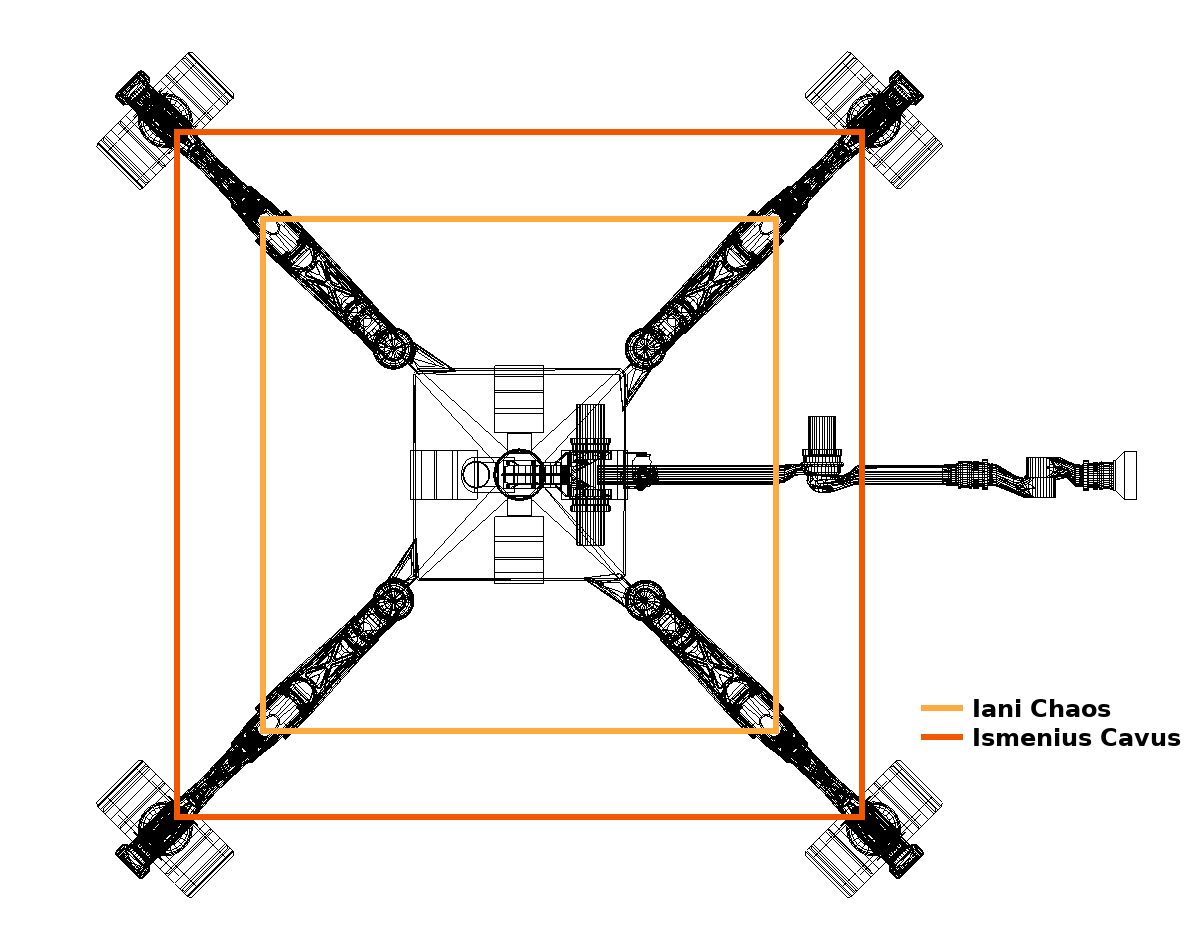
\includegraphics[width=0.8\linewidth]{sections/design/solar-array/images/sa-area-initial-sizes.png}\\
  \caption[Size comparison between SherpaTT and initial SA areas for Iani Chaos and Ismenius Cavus]
          {Size comparison between SherpaTT and initial \ac{SA} areas for Iani Chaos and Ismenius Cavus. The outlined square areas are equivalent to \ac{SA} areas of \SI{2.7}{m^{2}} for Iani Chaos and \SI{4.8}{m^{2}} for Ismenius Cavus.}
  \label{fig:sa-area-initial-sizes}
\end{figure}

To explain the lack of significant gain with $\beta_{best}$, the generated \ac{SA} energy and maximum traverse durations are plotted in Figures \ref{fig:plot:iani-chaos-generated-energy-and-max-traverse-durations} for Iani Chaos and Figure \ref{fig:plot:ismenius-cavus-generated-energy-and-max-traverse-durations} for Ismenius Cavus.

The \ref{itm:con:daylight_traverse} constraint imposed an upper limit to the maximum traverse durations. This ceiling corresponded to the daylight time that was available for traversing. At Iani Chaos, this resulted in the \ac{SA} generating excess propulsion energy which could not be used. For the scenario plotted in Figure \ref{fig:plot:sub:ismenius-cavus-max-traverse-durations}, this occured before and after the global storm season where both horizontal and $\beta_{best}$ inclined \ac{SA} surfaces generated excess energy which annulled any gains associated with solar tracking. This would have also have been the case during the global storm season for clear days with $\tau = 0.4$.

At Ismenius Cavus, the excess energy problem was further pronounced than in Iani Chaos. As seen in the scenario plotted in Figure \ref{fig:plot:sub:iani-chaos-max-traverse-durations}, an inclined \ac{SA} surface was only relevant during the global dust storm season with a dusty atmosphere of $\tau = 1$. This negligeable advantage resulted in the limited \SI{1.39}{\percent} traverse distance gain with $\beta_{best}$ that was noted earlier.

The \ac{SA} sizing using Equations \ref{calc:solar_cell_area_iani_chaos_traverse} and \ref{calc:solar_cell_area_ismenius_cavus_traverse} had to be approached differently to achieve significant gains with $\beta_{best}$ over a horizontal \ac{SA} surface, both in terms of \ac{SA} area reduction and in attainable traverse distances. Lack of appreciable distance coverage gains with $\beta_{best}$ lies in the optical depths that were used to determine $H_{\beta}^{worst}$ with $\tau = 1$. For high $\tau$ factors, $H_{\beta}^{worst} \approx H_{h}^{worst}$ due to light scattering by airborn Martian dust. This was previously observed in Figure \ref{fig:plot:insolation-ls}, where diffuse insolation was already the largest component contributing to global insolation at $\tau = 1$. Inclined \ac{SA} surface yield little to no benefits over horizontal surfaces when light is mostly diffuse.

\begin{figure}[h]
\captionsetup[subfigure]{justification=centering}
\vspace{-2ex}
	\centering
    %% setup sizes
    \setlength{\subfigureWidth}{0.50\textwidth}
    \setlength{\graphicsHeight}{80mm}
    %% kill hyper-link highlighting
    \hypersetup{hidelinks=true}%
    %% the figures
    \begin{subfigure}[t]{\subfigureWidth}
        \centering
        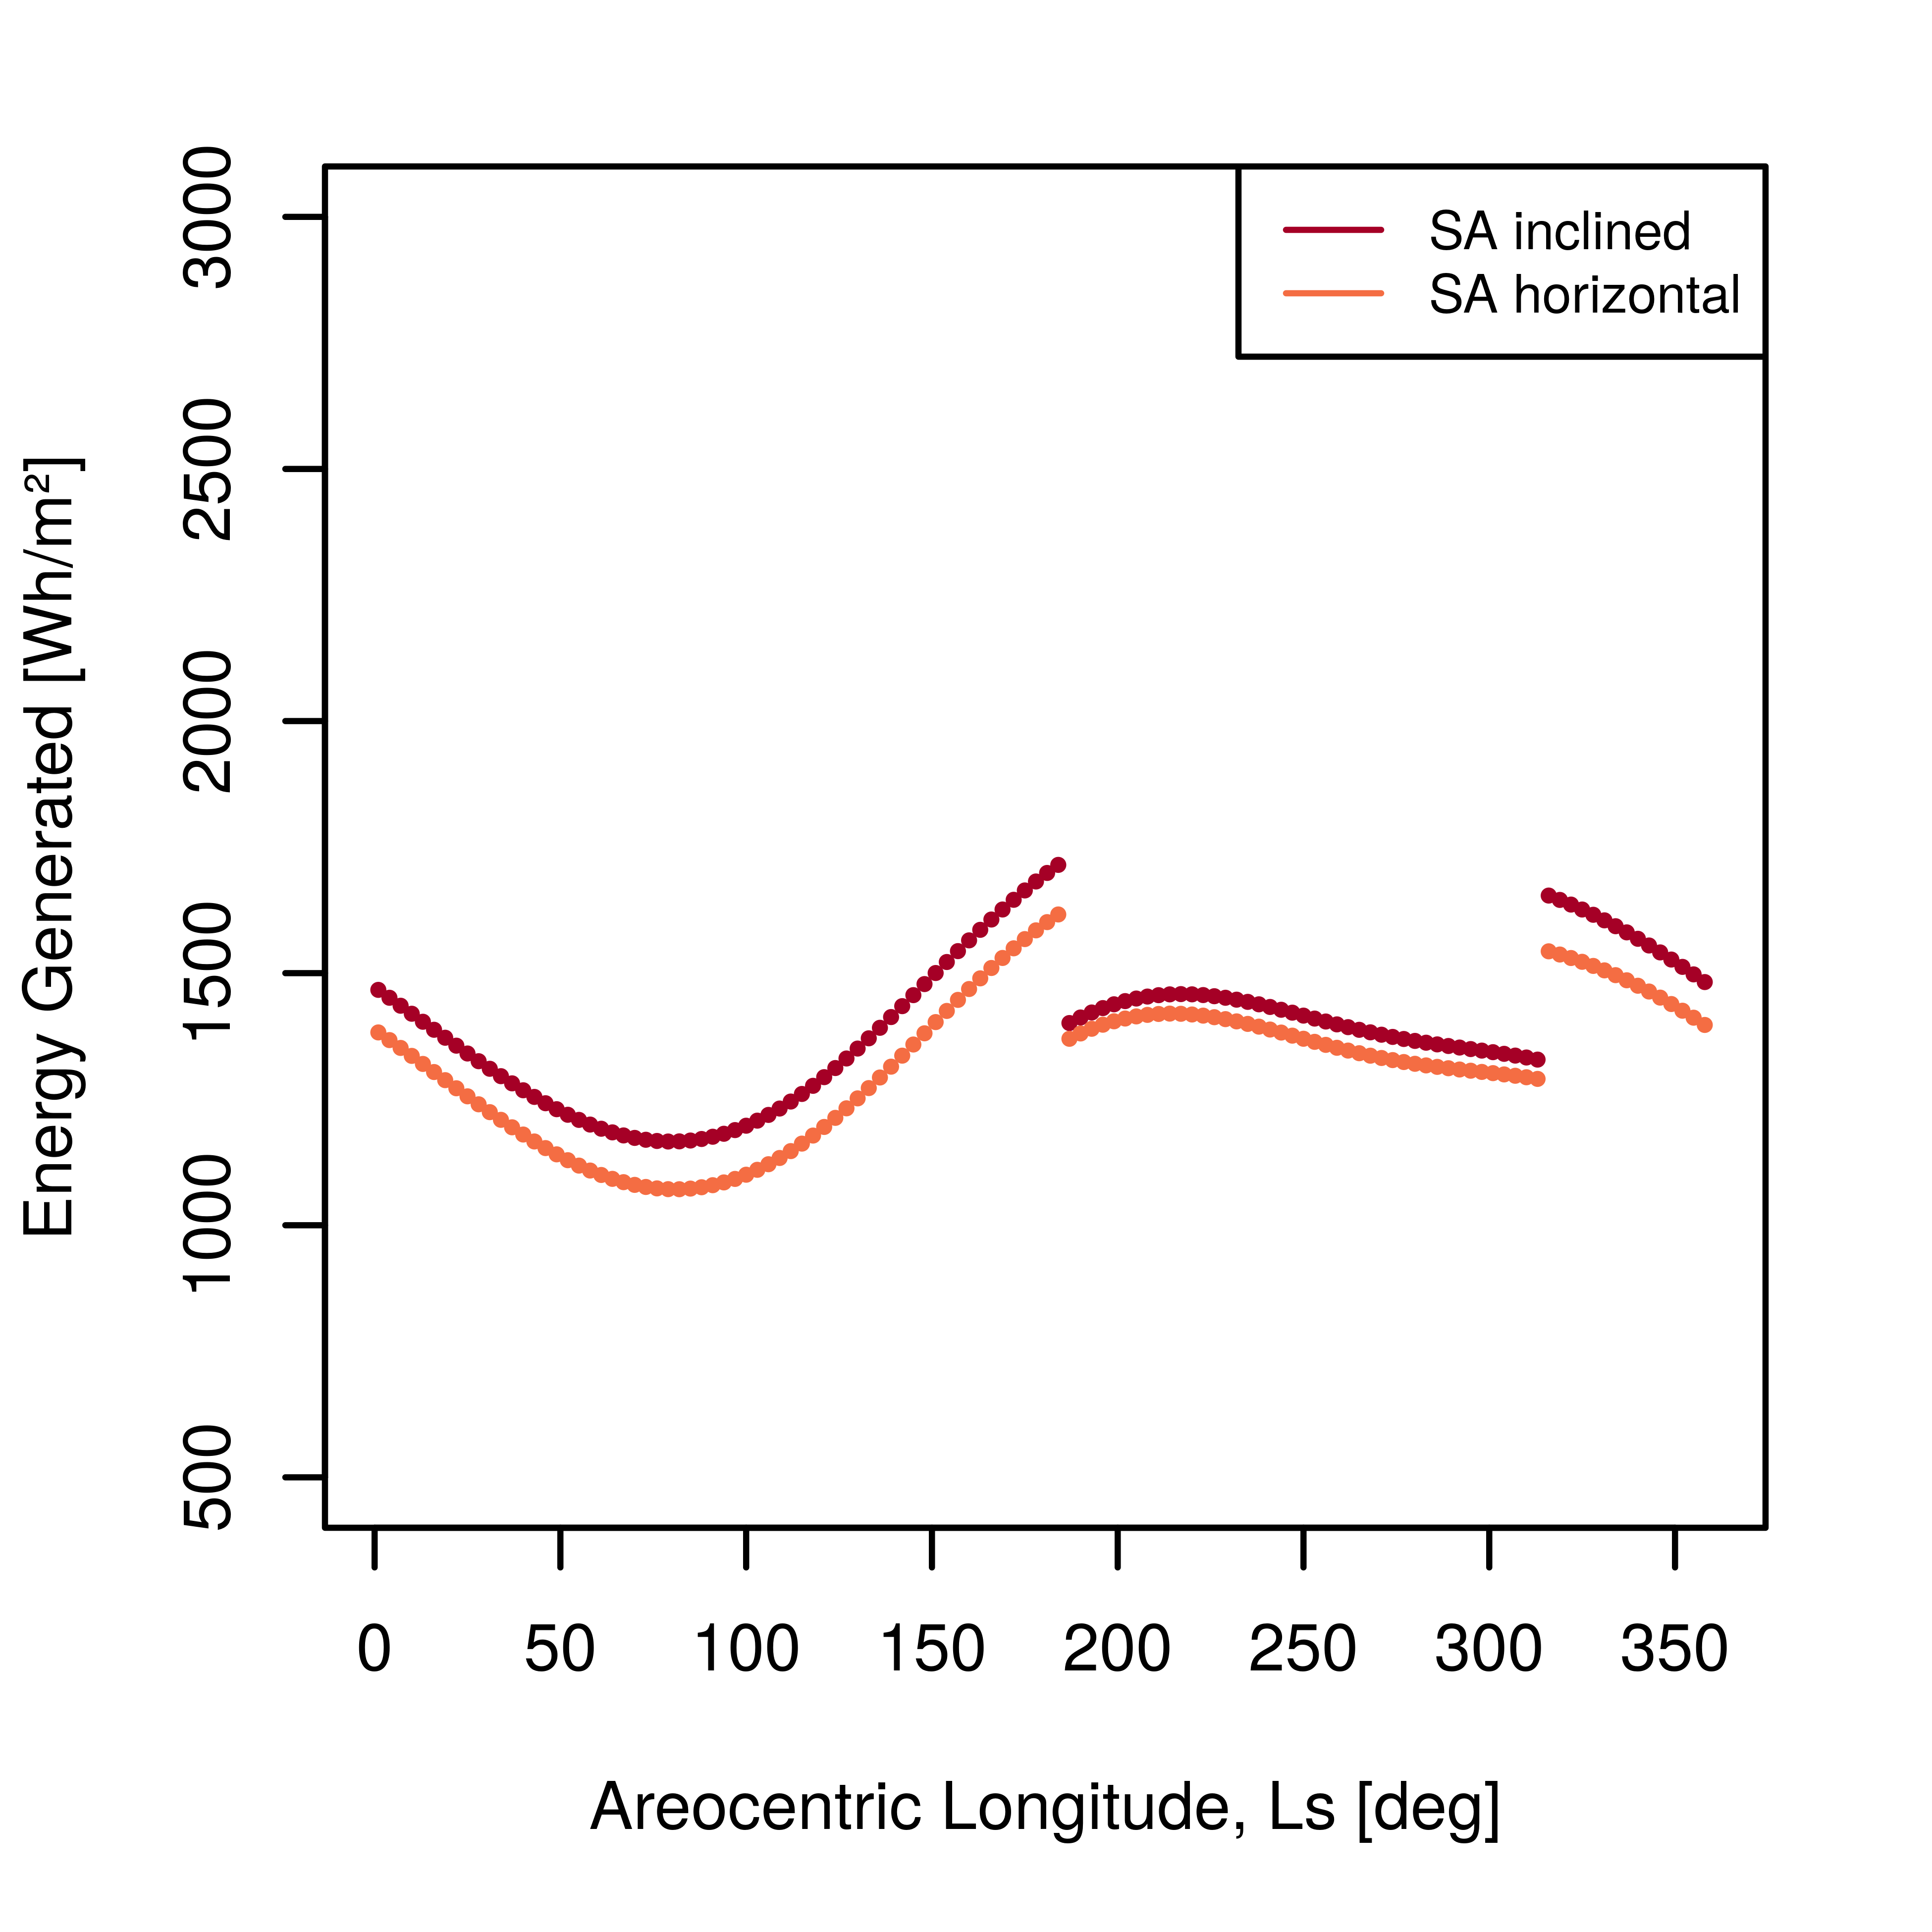
\includegraphics[height=\graphicsHeight]{sections/design/solar-array/plots/ianichaos-daily-generated-energy-for-sa-area-27m2.png}
        \subcaption{Generated Energy}
        \label{fig:plot:sub:iani-chaos-generated-energy}
    \end{subfigure}\hfill
    \begin{subfigure}[t]{\subfigureWidth}
        \centering
        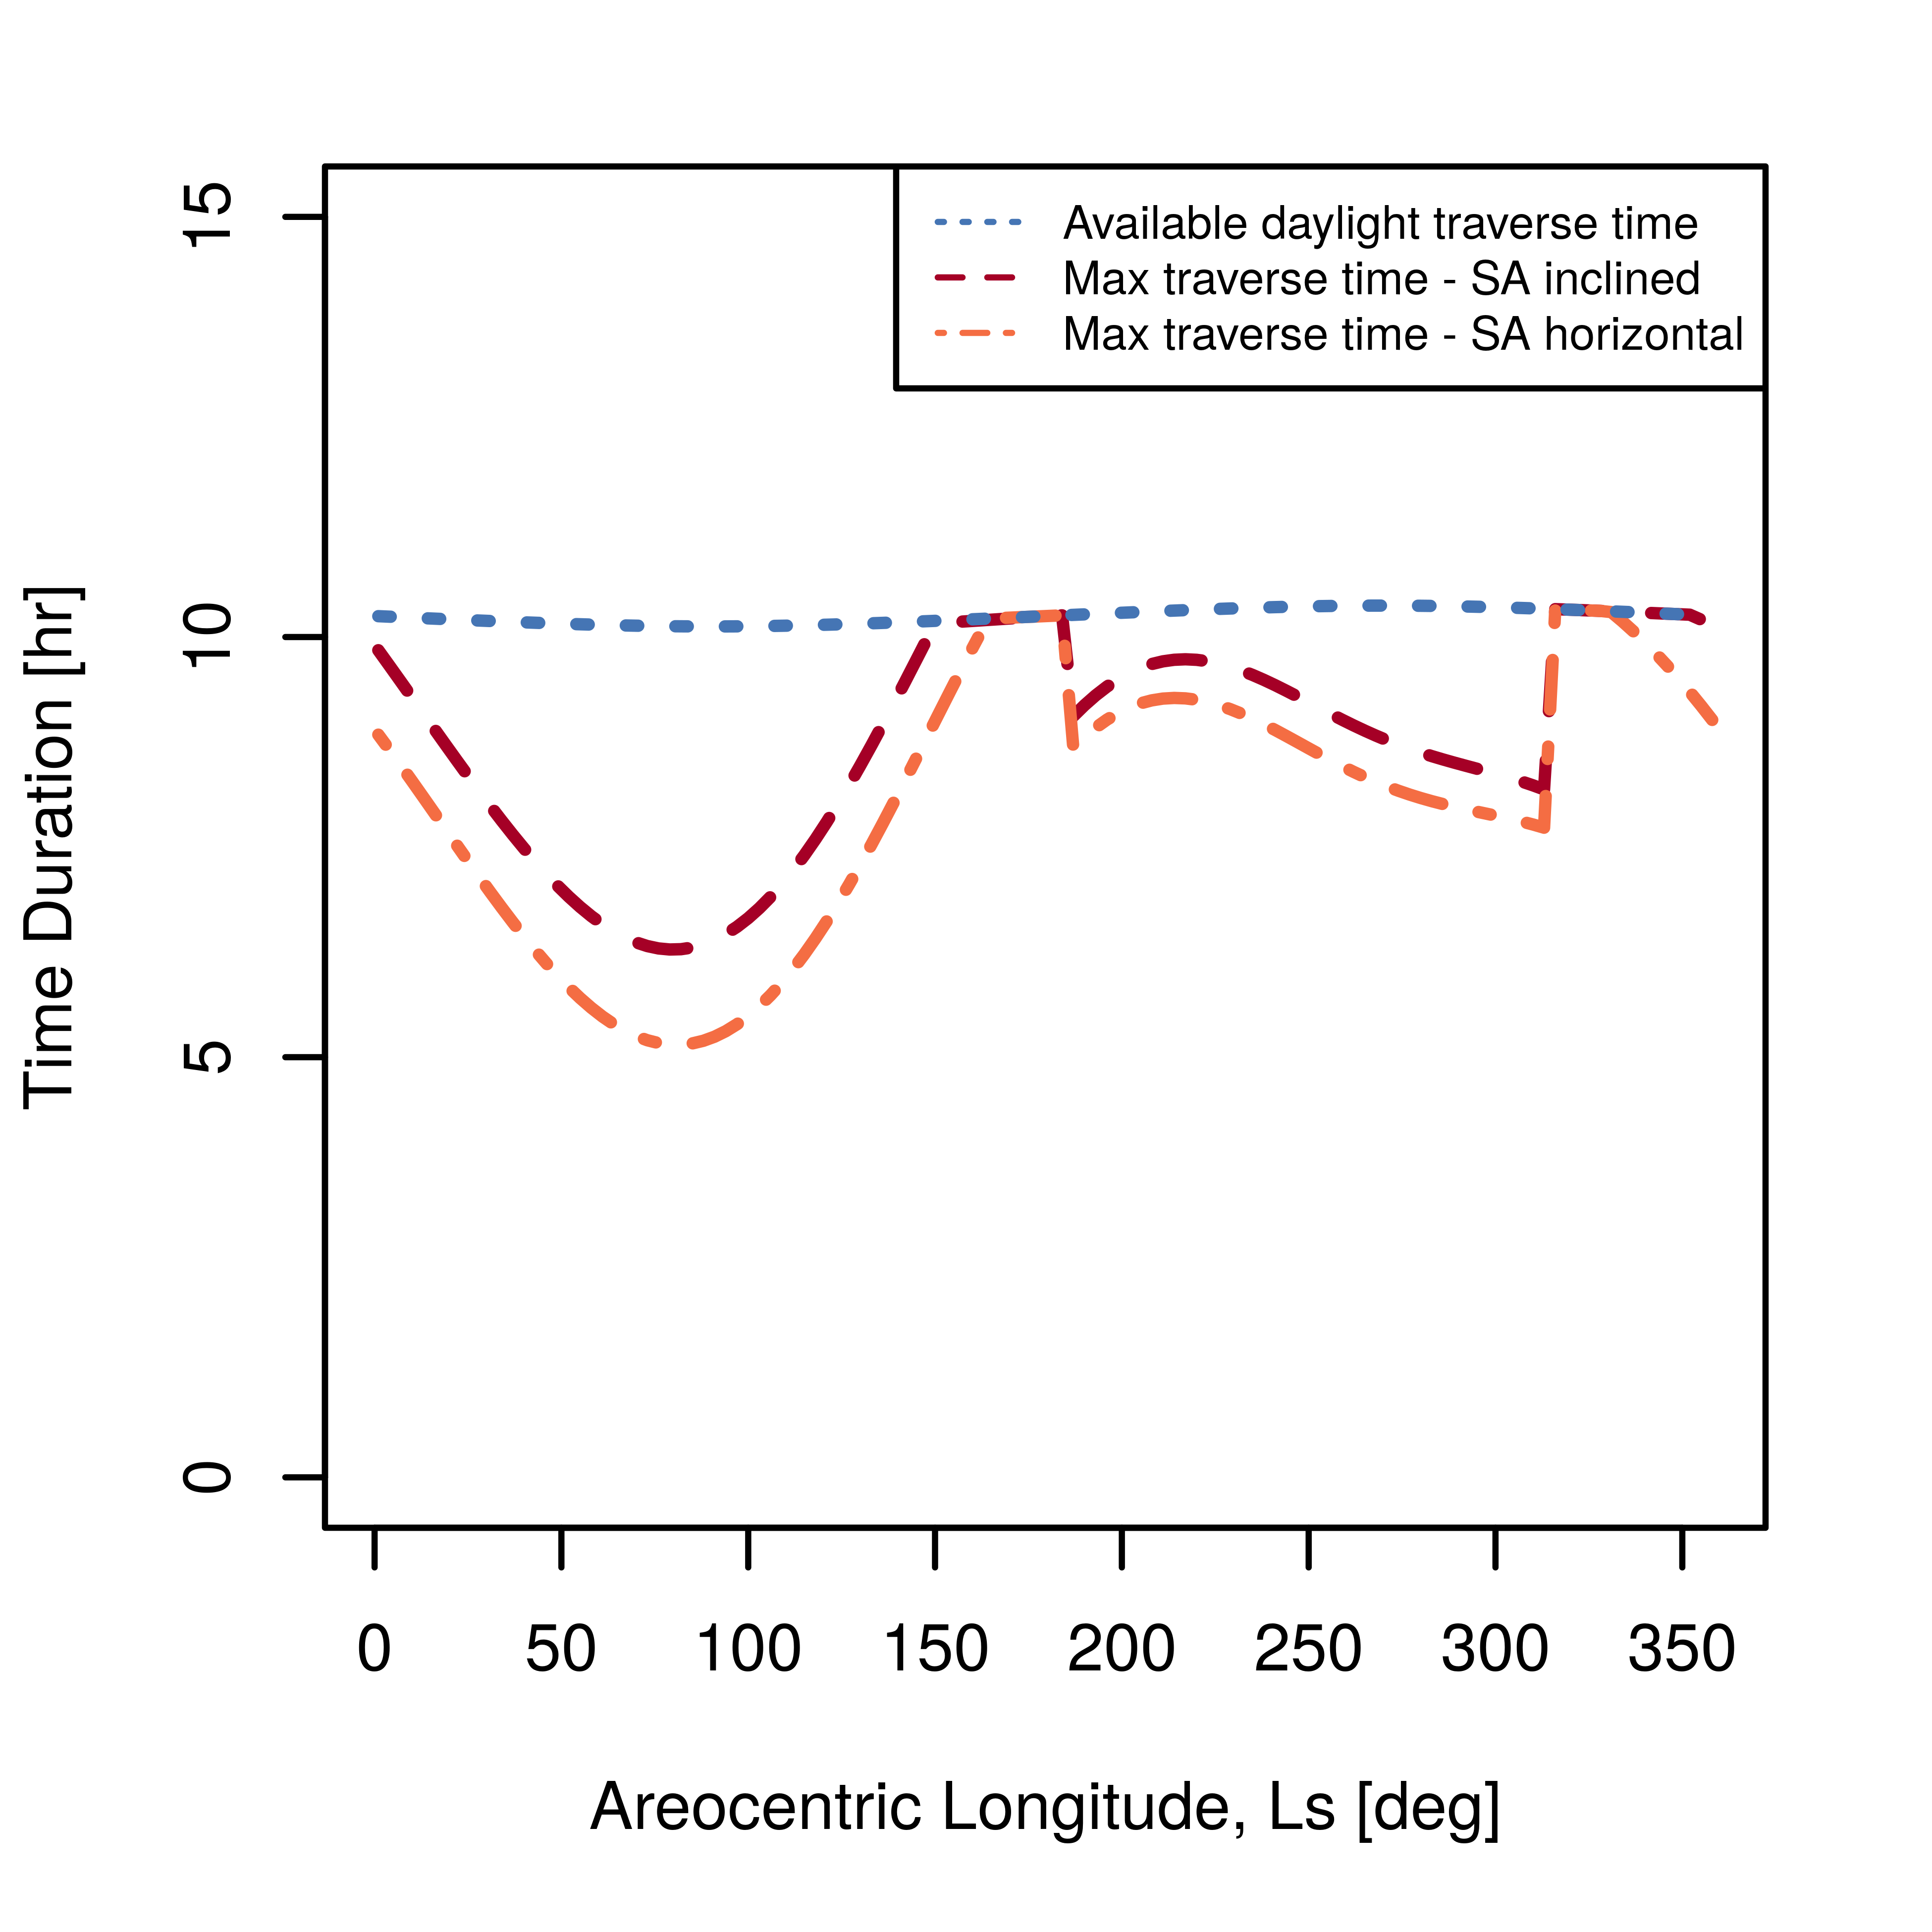
\includegraphics[height=\graphicsHeight]{sections/design/solar-array/plots/ianichaos-75w-max-traverse-durations-for-sa-area-27m2.png}
  		\subcaption{Maximum Traverse Durations}
		\label{fig:plot:sub:iani-chaos-max-traverse-durations}
	\end{subfigure}\\[0.8ex]
    \caption[Generated energy and maxium achievable flat terrain traverse durations at Iani Chaos]
            {Generated energy and maxium achievable flat terrain traverse duration at Iani Chaos with \ac{SA} area = \SI{2.7}{m^{2}}. Optical depth  $\tau = 1$ was used for global dust storm season ($\SI{185}{\degree} \leq L_{s} \leq \SI{315}{\degree}$) and $\tau = 0.4$ for the remainder of the year. The \textit{available daylight traverse time} corresponds to the amount of daylight hours left in a \textit{Traverse Sol} after subtracting the time taken by non-Traverse modes: \textit{Idle - Day}, \textit{\ac{DTE} Communication}, \textit{Science Stop - Short}, and \textit{Optimal Pose}. The maximum traverse durations for \ac{SA} horizontal do not consider the \textit{Optimal Pose} mode.}
    \label{fig:plot:iani-chaos-generated-energy-and-max-traverse-durations}
\vspace{-2ex}
\end{figure}

\begin{figure}[h]
\captionsetup[subfigure]{justification=centering}
\vspace{-2ex}
	\centering
    %% setup sizes
    \setlength{\subfigureWidth}{0.50\textwidth}
    \setlength{\graphicsHeight}{80mm}
    %% kill hyper-link highlighting
    \hypersetup{hidelinks=true}%
    %% the figures
    \begin{subfigure}[t]{\subfigureWidth}
        \centering
        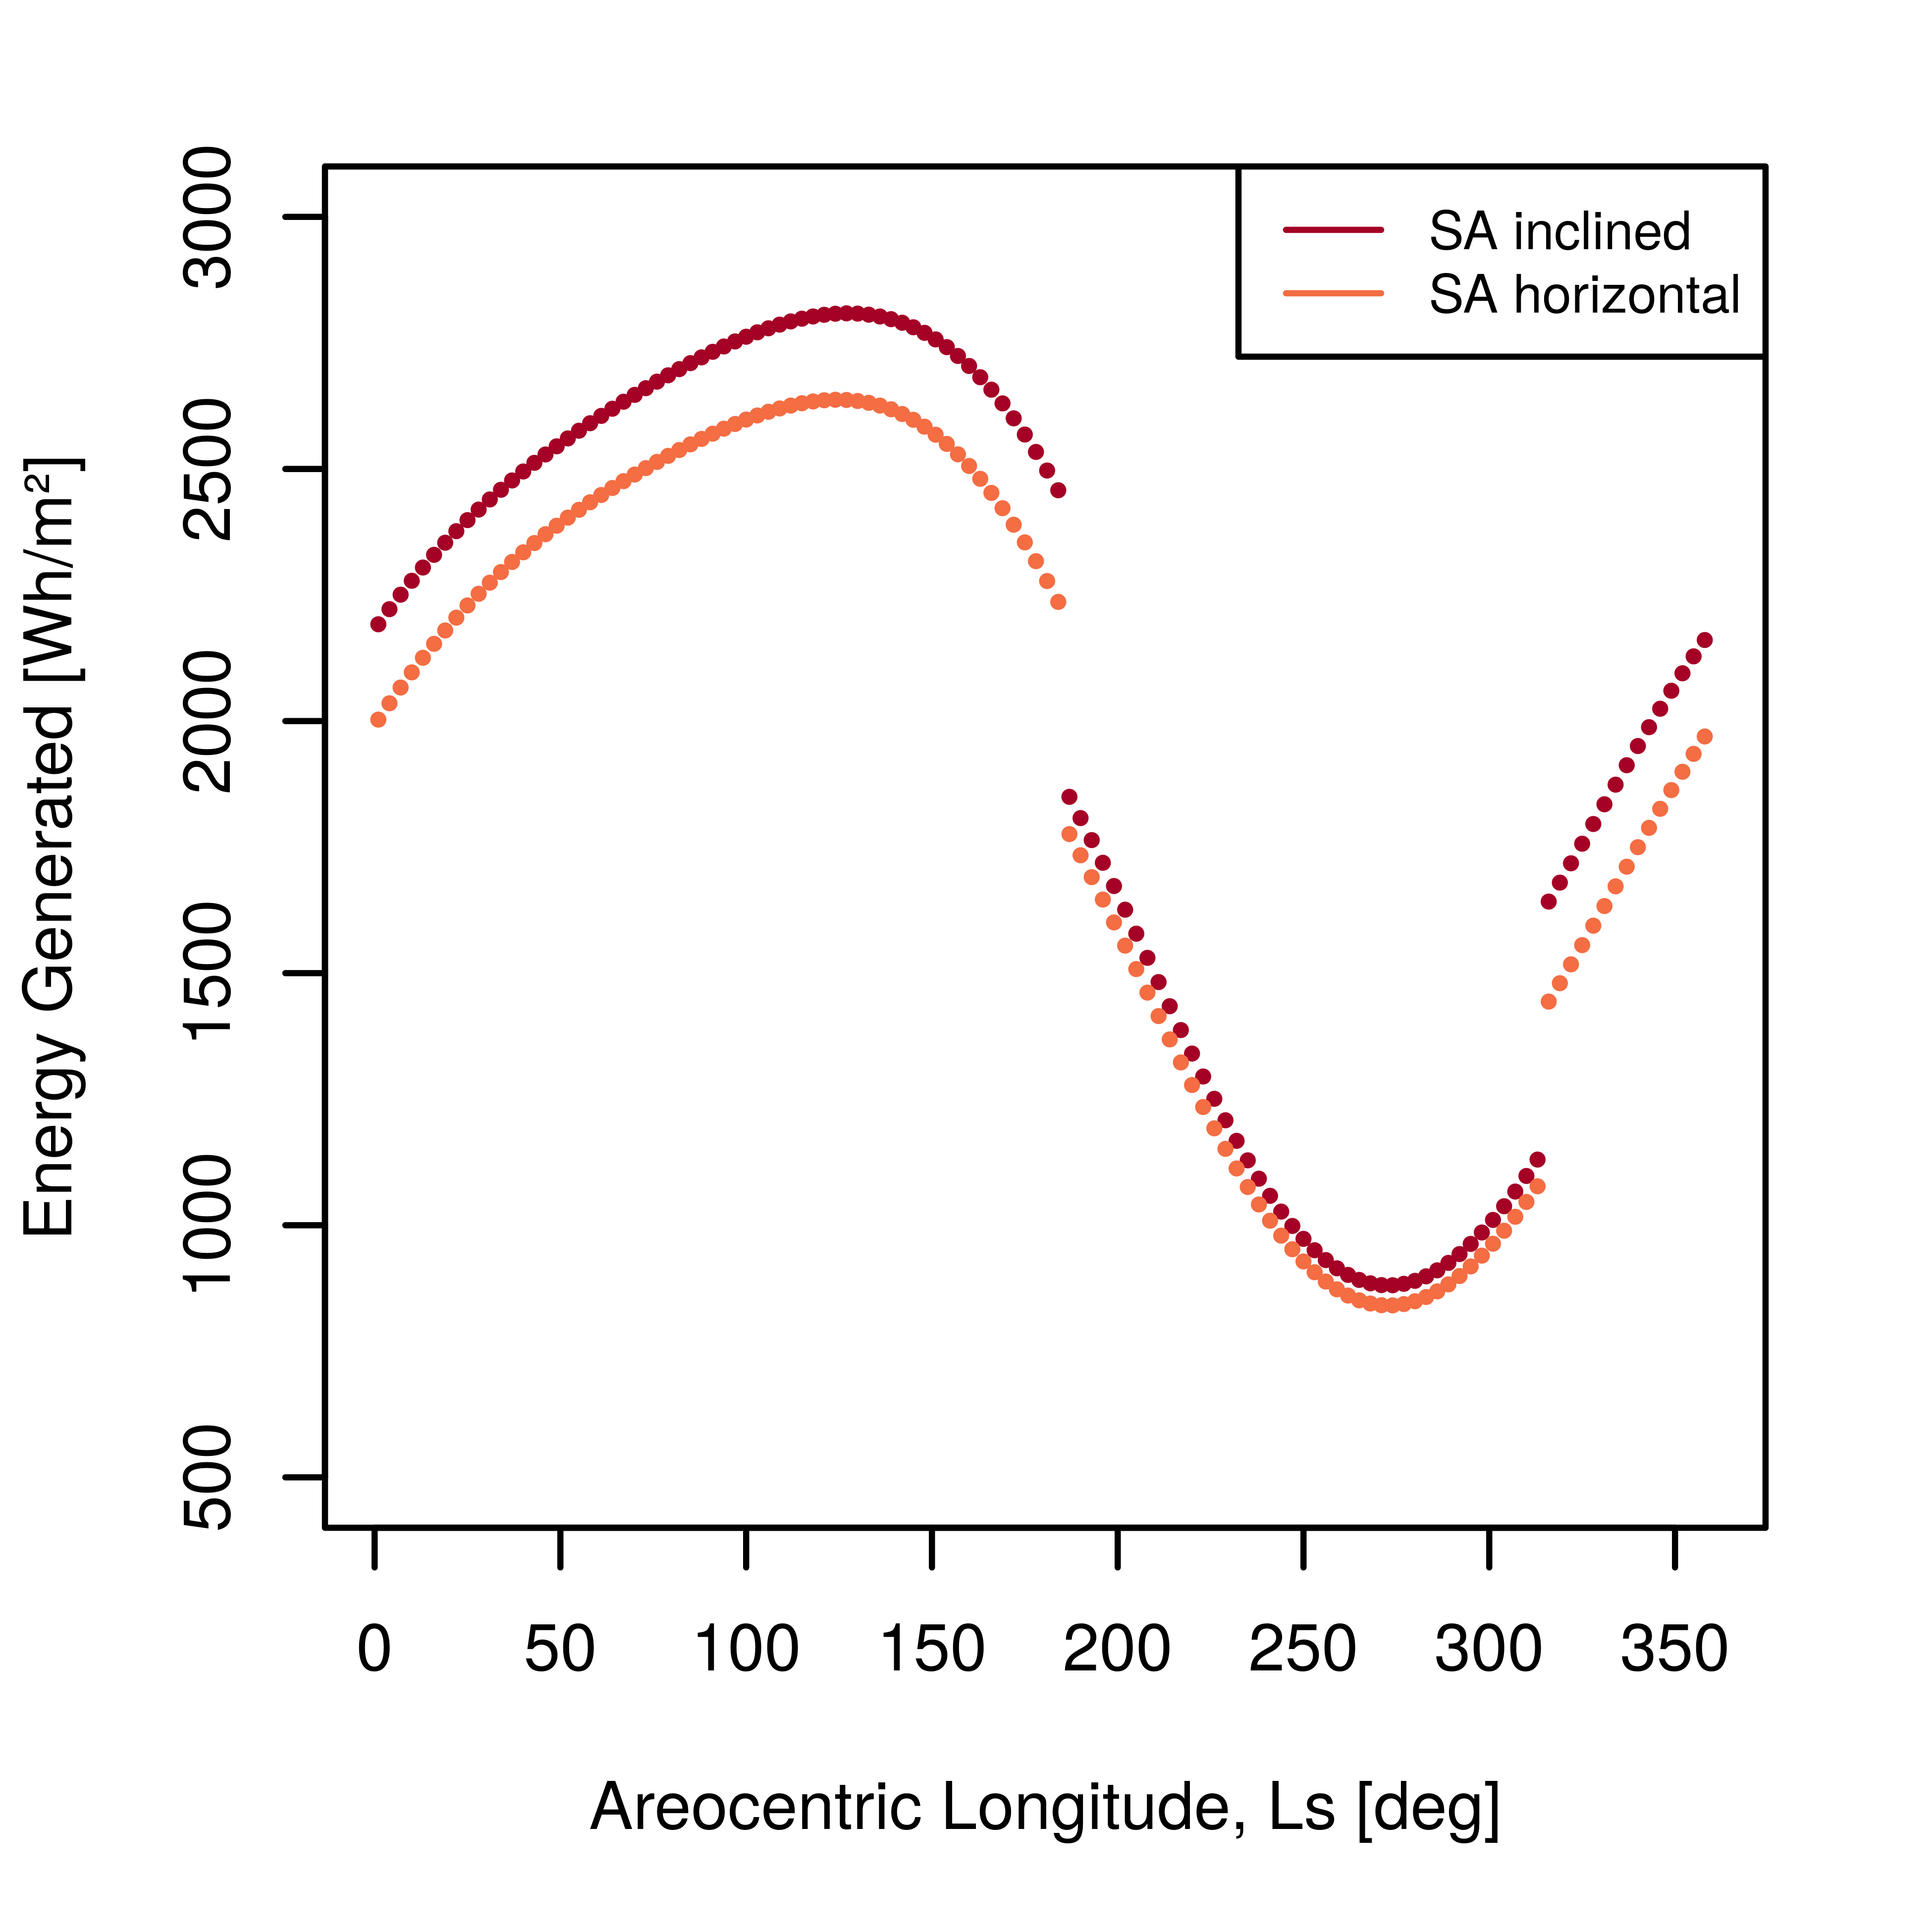
\includegraphics[height=\graphicsHeight]{sections/design/solar-array/plots/ismeniuscavus-daily-generated-energy-for-sa-area-48m2.png}
        \subcaption{Generated Energy}
        \label{fig:plot:sub:ismenius-cavus-generated-energy}
    \end{subfigure}\hfill
    \begin{subfigure}[t]{\subfigureWidth}
        \centering
        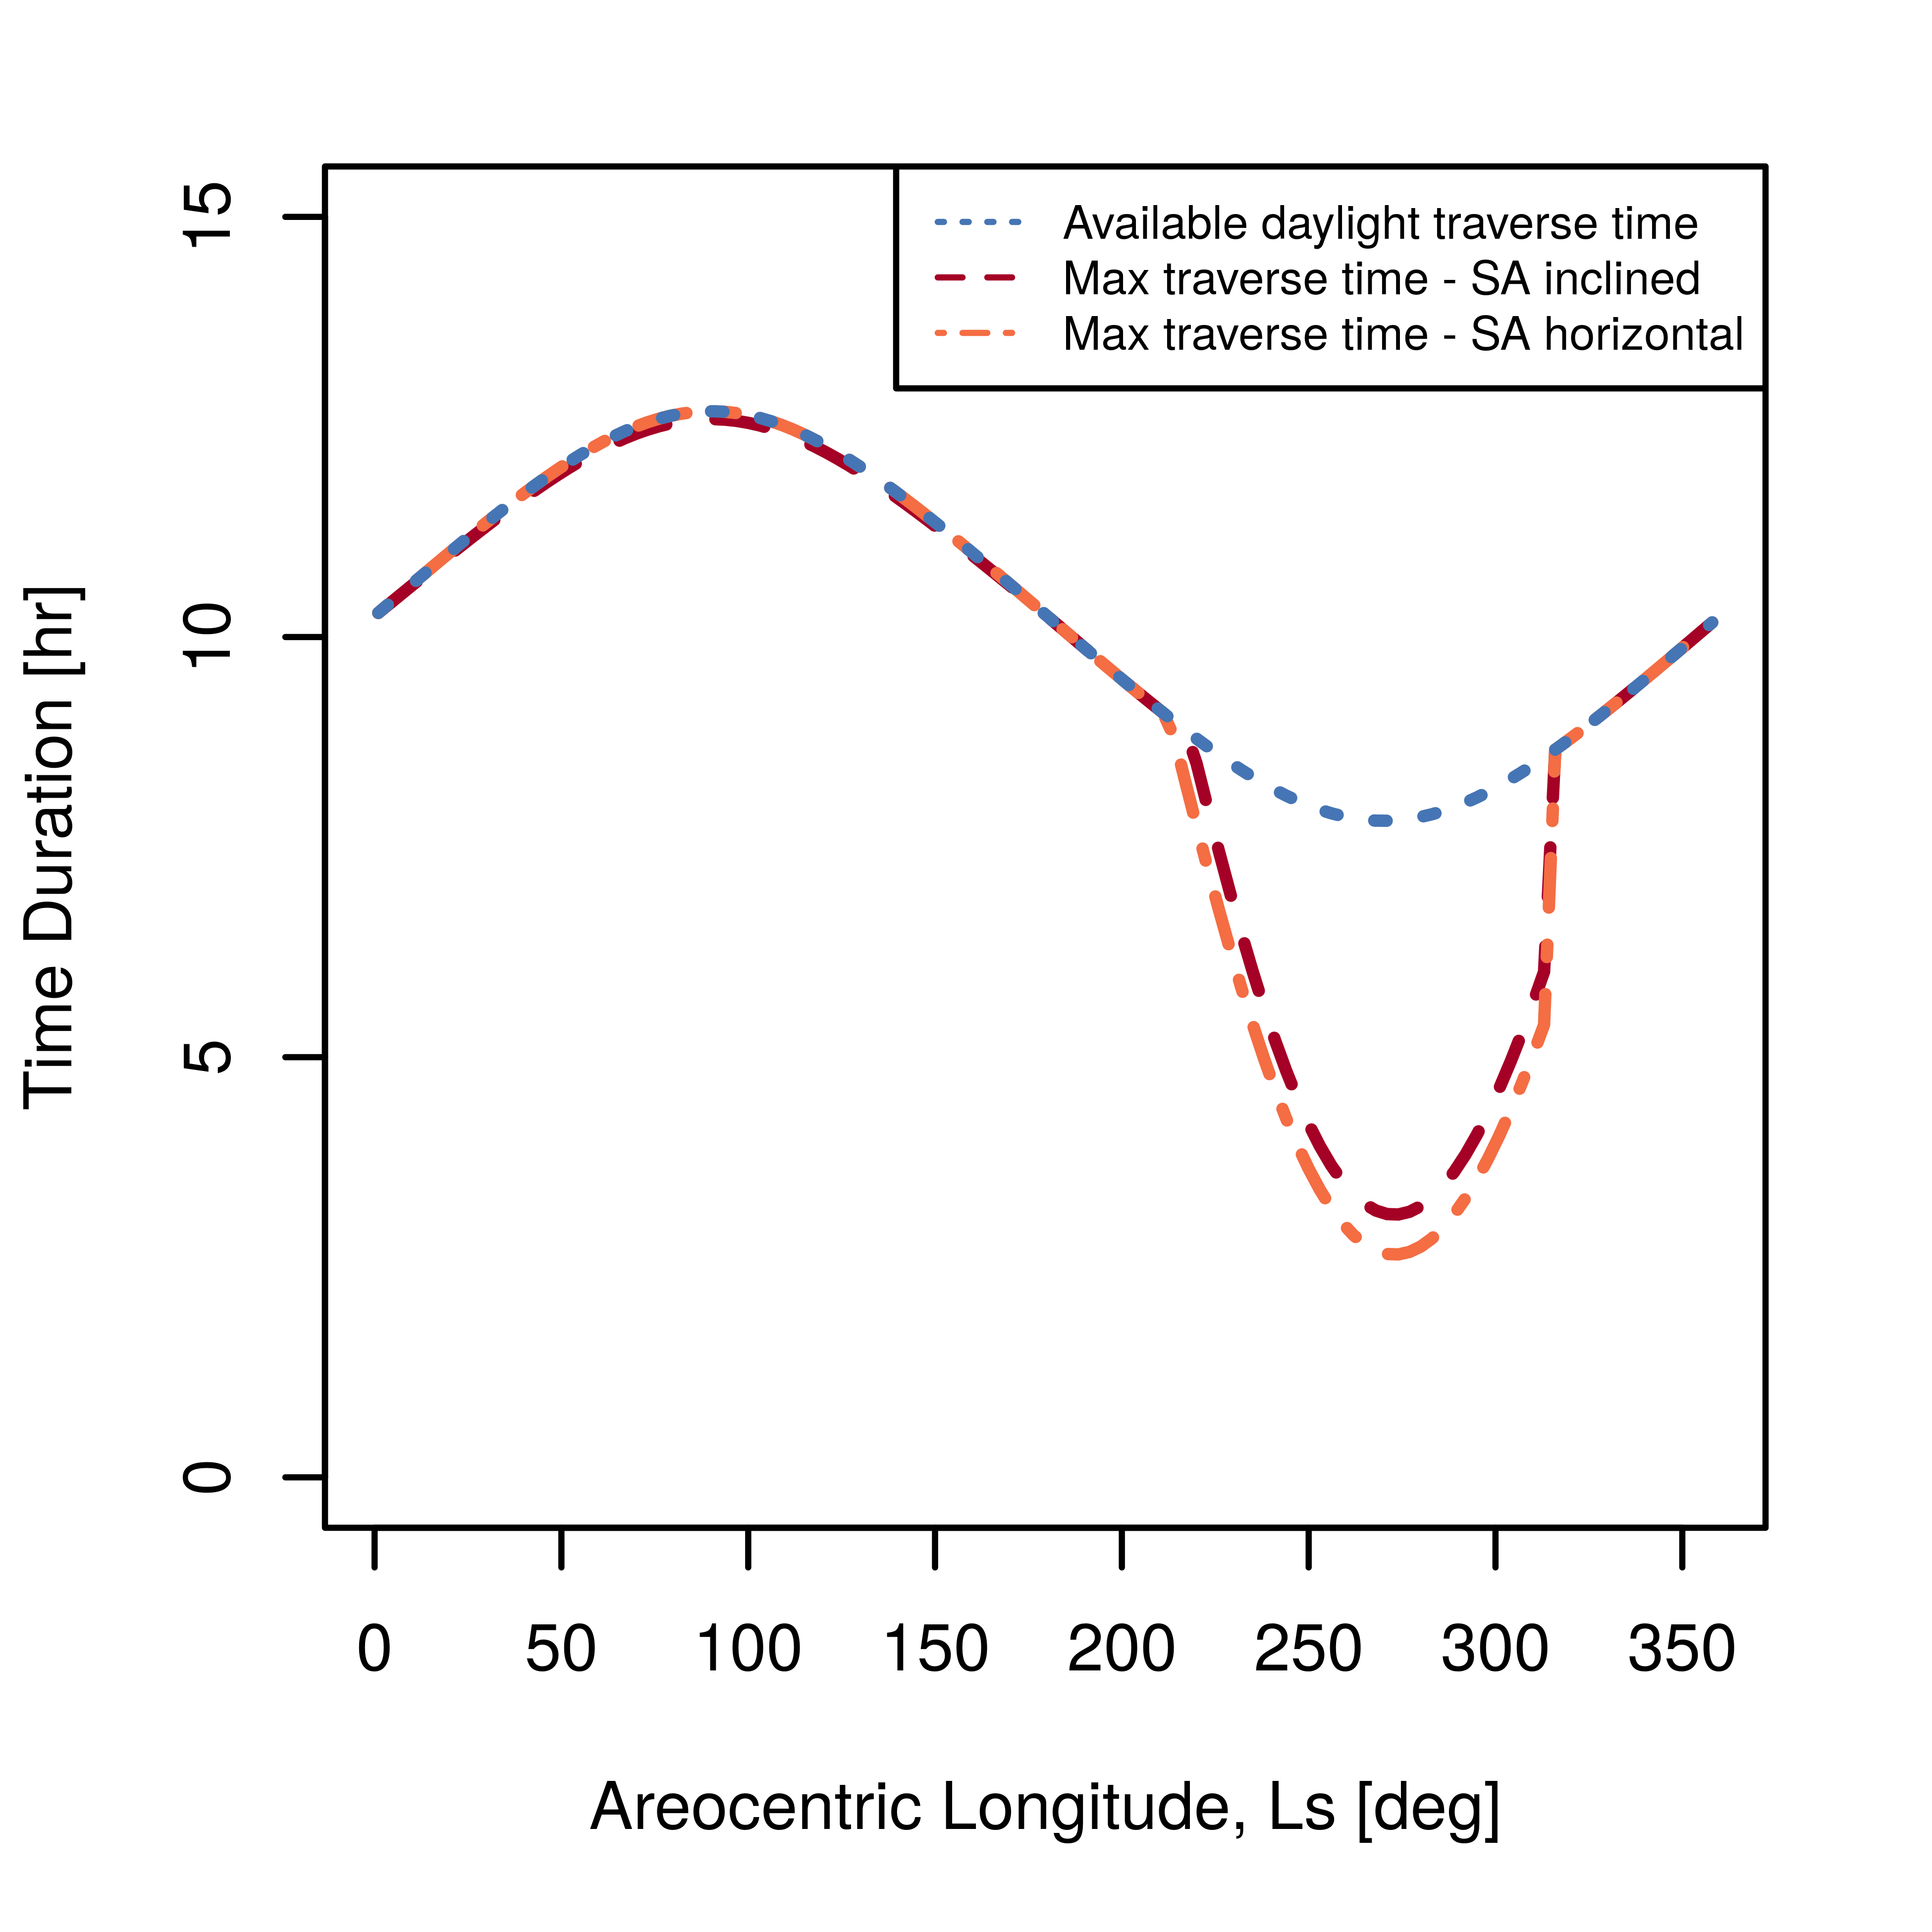
\includegraphics[height=\graphicsHeight]{sections/design/solar-array/plots/ismeniuscavus-75w-max-traverse-durations-for-sa-area-48m2.png}
  		\subcaption{Maximum Traverse Durations}
		\label{fig:plot:sub:ismenius-cavus-max-traverse-durations}
	\end{subfigure}\\[0.8ex]
    \caption[Generated energy and maxium achievable flat terrain traverse durations at Ismenius Cavus]
            {Generated energy and maxium achievable flat terrain traverse duration at Ismenius Cavus with \ac{SA} area = \SI{4.8}{m^{2}}. The same considerations were taken as in Figure \ref{fig:plot:iani-chaos-generated-energy-and-max-traverse-durations}.}
    \label{fig:plot:ismenius-cavus-generated-energy-and-max-traverse-durations}
\vspace{-2ex}
\end{figure}

\clearpage
\ac{SA} sizes of \SI{2.7}{m^{2}} at Iani Chaos and \SI{4.8}{m^{2}} at Ismenius Cavus resulted in total attainable distance coverages of \SI{64}{\kilo\meter} and \SI{68}{\kilo\meter} of flat traverses within one \ac{MY}. These distances exceeded by over threefolds the \ref{itm:req:total_distance_flat_terrain} requirement of \SI{20}{\kilo\meter}. $E_{req}^{worst}$ was changed from energy required for the worst case \textit{Traverse Sol} to energy required for a \textit{Hibernation Sol}. To attain satisfying results the solar power draw required by the \textit{Hibernation mode} needed to be reduced from \SI{18}{\watt} to \SI{17}{\watt} at Iani Chaos and from \SI{18}{\watt} to \SI{15}{\watt} at Ismenius Cavus. Introducing \acp{RHU} will be necessary should these revised solar power requirements be unachievable. A single \ac{RHU} provides approximately \SI{1}{\watt} of heat thus one \ac{RHU} would be required at Iani Chaos and three at Ismenius Cavus. After taking into account a \SI{20}{percent} system margin, $E_{req}^{worst}$ became \SI{490}{\watt\hour} for a \textit{Hibernation Sol} at Iani Chaos and \SI{432}{\watt\hour} at Ismenius Cavus. Revisting Equation \ref{eq:solar_cell_coverage_area} resulted in the following solar cell coverage areas:


\begin{align}
  \label{calc:solar_cell_area_iani_chaos_hibernation}
  A_{iani} &= \frac{E_{req}^{worst}}{\eta_{EOL} \cdot H_{\beta}^{worst} \cdot PR_{EOL}}\\
           &= \frac{490}{0.22 \cdot 2479 \cdot 0.62}\\
           &= \SI{1.45}{m^{2}}
\end{align}

\begin{align}
  \label{calc:solar_cell_area_ismenius_cavus_hibernation}
  A_{ismenius} &= \frac{E_{req}^{worst}}{\eta_{EOL} \cdot H_{\beta}^{worst} \cdot PR_{EOL}}\\
               &= \frac{432}{0.22 \cdot 1345 \cdot 0.62}\\
               &= \SI{2.35}{m^{2}}
\end{align}

After considering \ref{itm:ass:packing_efficiency}, the \ac{SA} area were \SI{1.7}{m^{2}} at Iani Chaos with a mass of \SI{6.3}{\kilo\gram} and \SI{2.8}{m^{2}} at Ismenius Cavus with a mass of  \SI{10.4}{\kilo\gram}. The \ref{itm:req:total_distance_flat_terrain} requirement remained satisfied with
a maxmium flat traverse distance coverage of \SI{21}{\kilo\meter} at Iani Chaos and \SI{48}{\kilo\meter} at Ismenius Cavus. Figure \ref{fig:plot:flat-traverse-gains-for-different-sa-area} compares the gains in flat traverse distance coverage for different \ac{SA} sizes and optical depths so that the relationship between \ac{SA} area and benefits of solar tracking may be further appreciated. At Iani Chaos, a \SI{26}{\percent} gain in flat traverse distance coverage was achieved with a $\beta_{best}$ inclined surface during a clear day with $\tau = 0.4$. On a dusty day with $\tau = 1$, this gain was still significant at \SI{14}{\percent}. At Ismenius cavus, $\tau = 0.4$ and $\tau = 1$ gains are \SI{21}{\percent} and \SI{9}{\percent}, respectively. The maximum daily traverse durations attainable at both sites with their respective \ac{SA} sizes are shown in Figure \ref{fig:plot:final-maximum-traverse-durations-at-missions-sites}.


\begin{figure}[h]
\captionsetup[subfigure]{justification=centering}
\vspace{-2ex}
	\centering
    %% setup sizes
    \setlength{\subfigureWidth}{0.50\textwidth}
    \setlength{\graphicsHeight}{80mm}
    %% kill hyper-link highlighting
    \hypersetup{hidelinks=true}%
    %% the figures
    \begin{subfigure}[t]{\subfigureWidth}
        \centering
        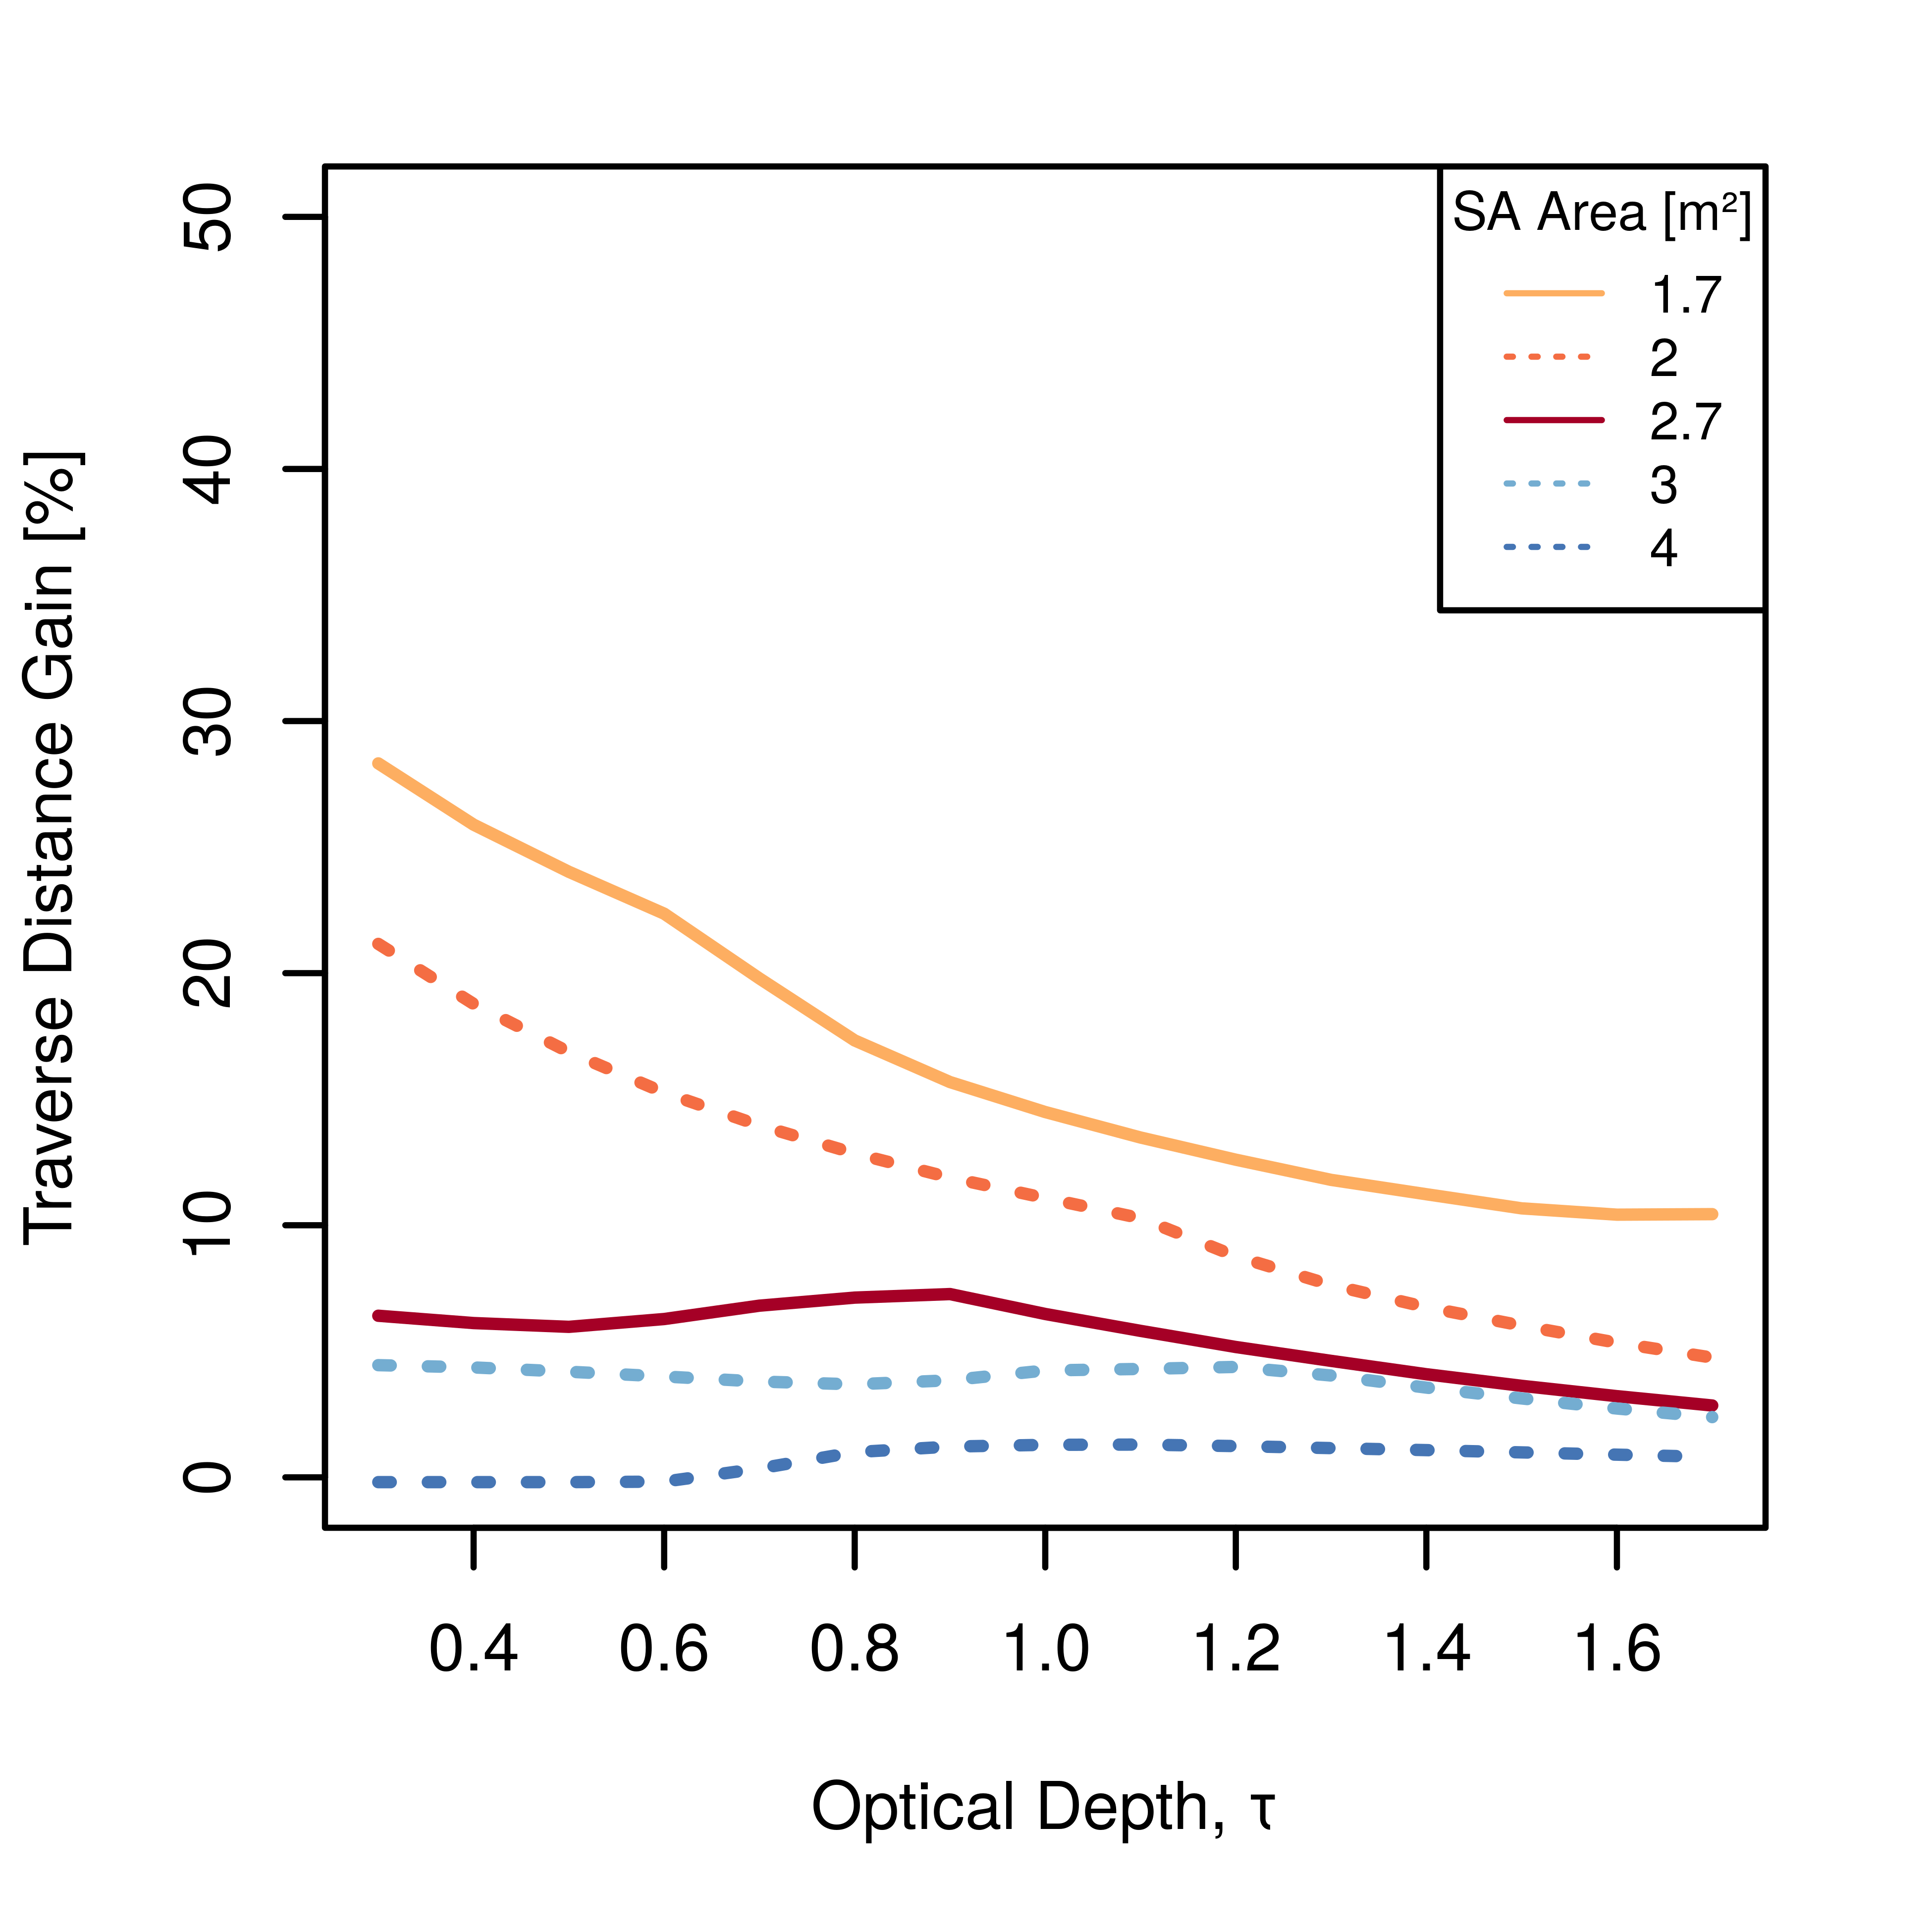
\includegraphics[height=\graphicsHeight]{sections/design/solar-array/plots/ianichaos-75w-traverse-gains-for-different-sa-areas.png}
  		\subcaption{Iani Chaos, \ac{SA} area = \SI{1.7}{m^{2}}}
		\label{fig:plot:sub:ismenius-chaos-flat-traverse-gains-for-different-sa-area}
    \end{subfigure}\hfill
    \begin{subfigure}[t]{\subfigureWidth}
        \centering
        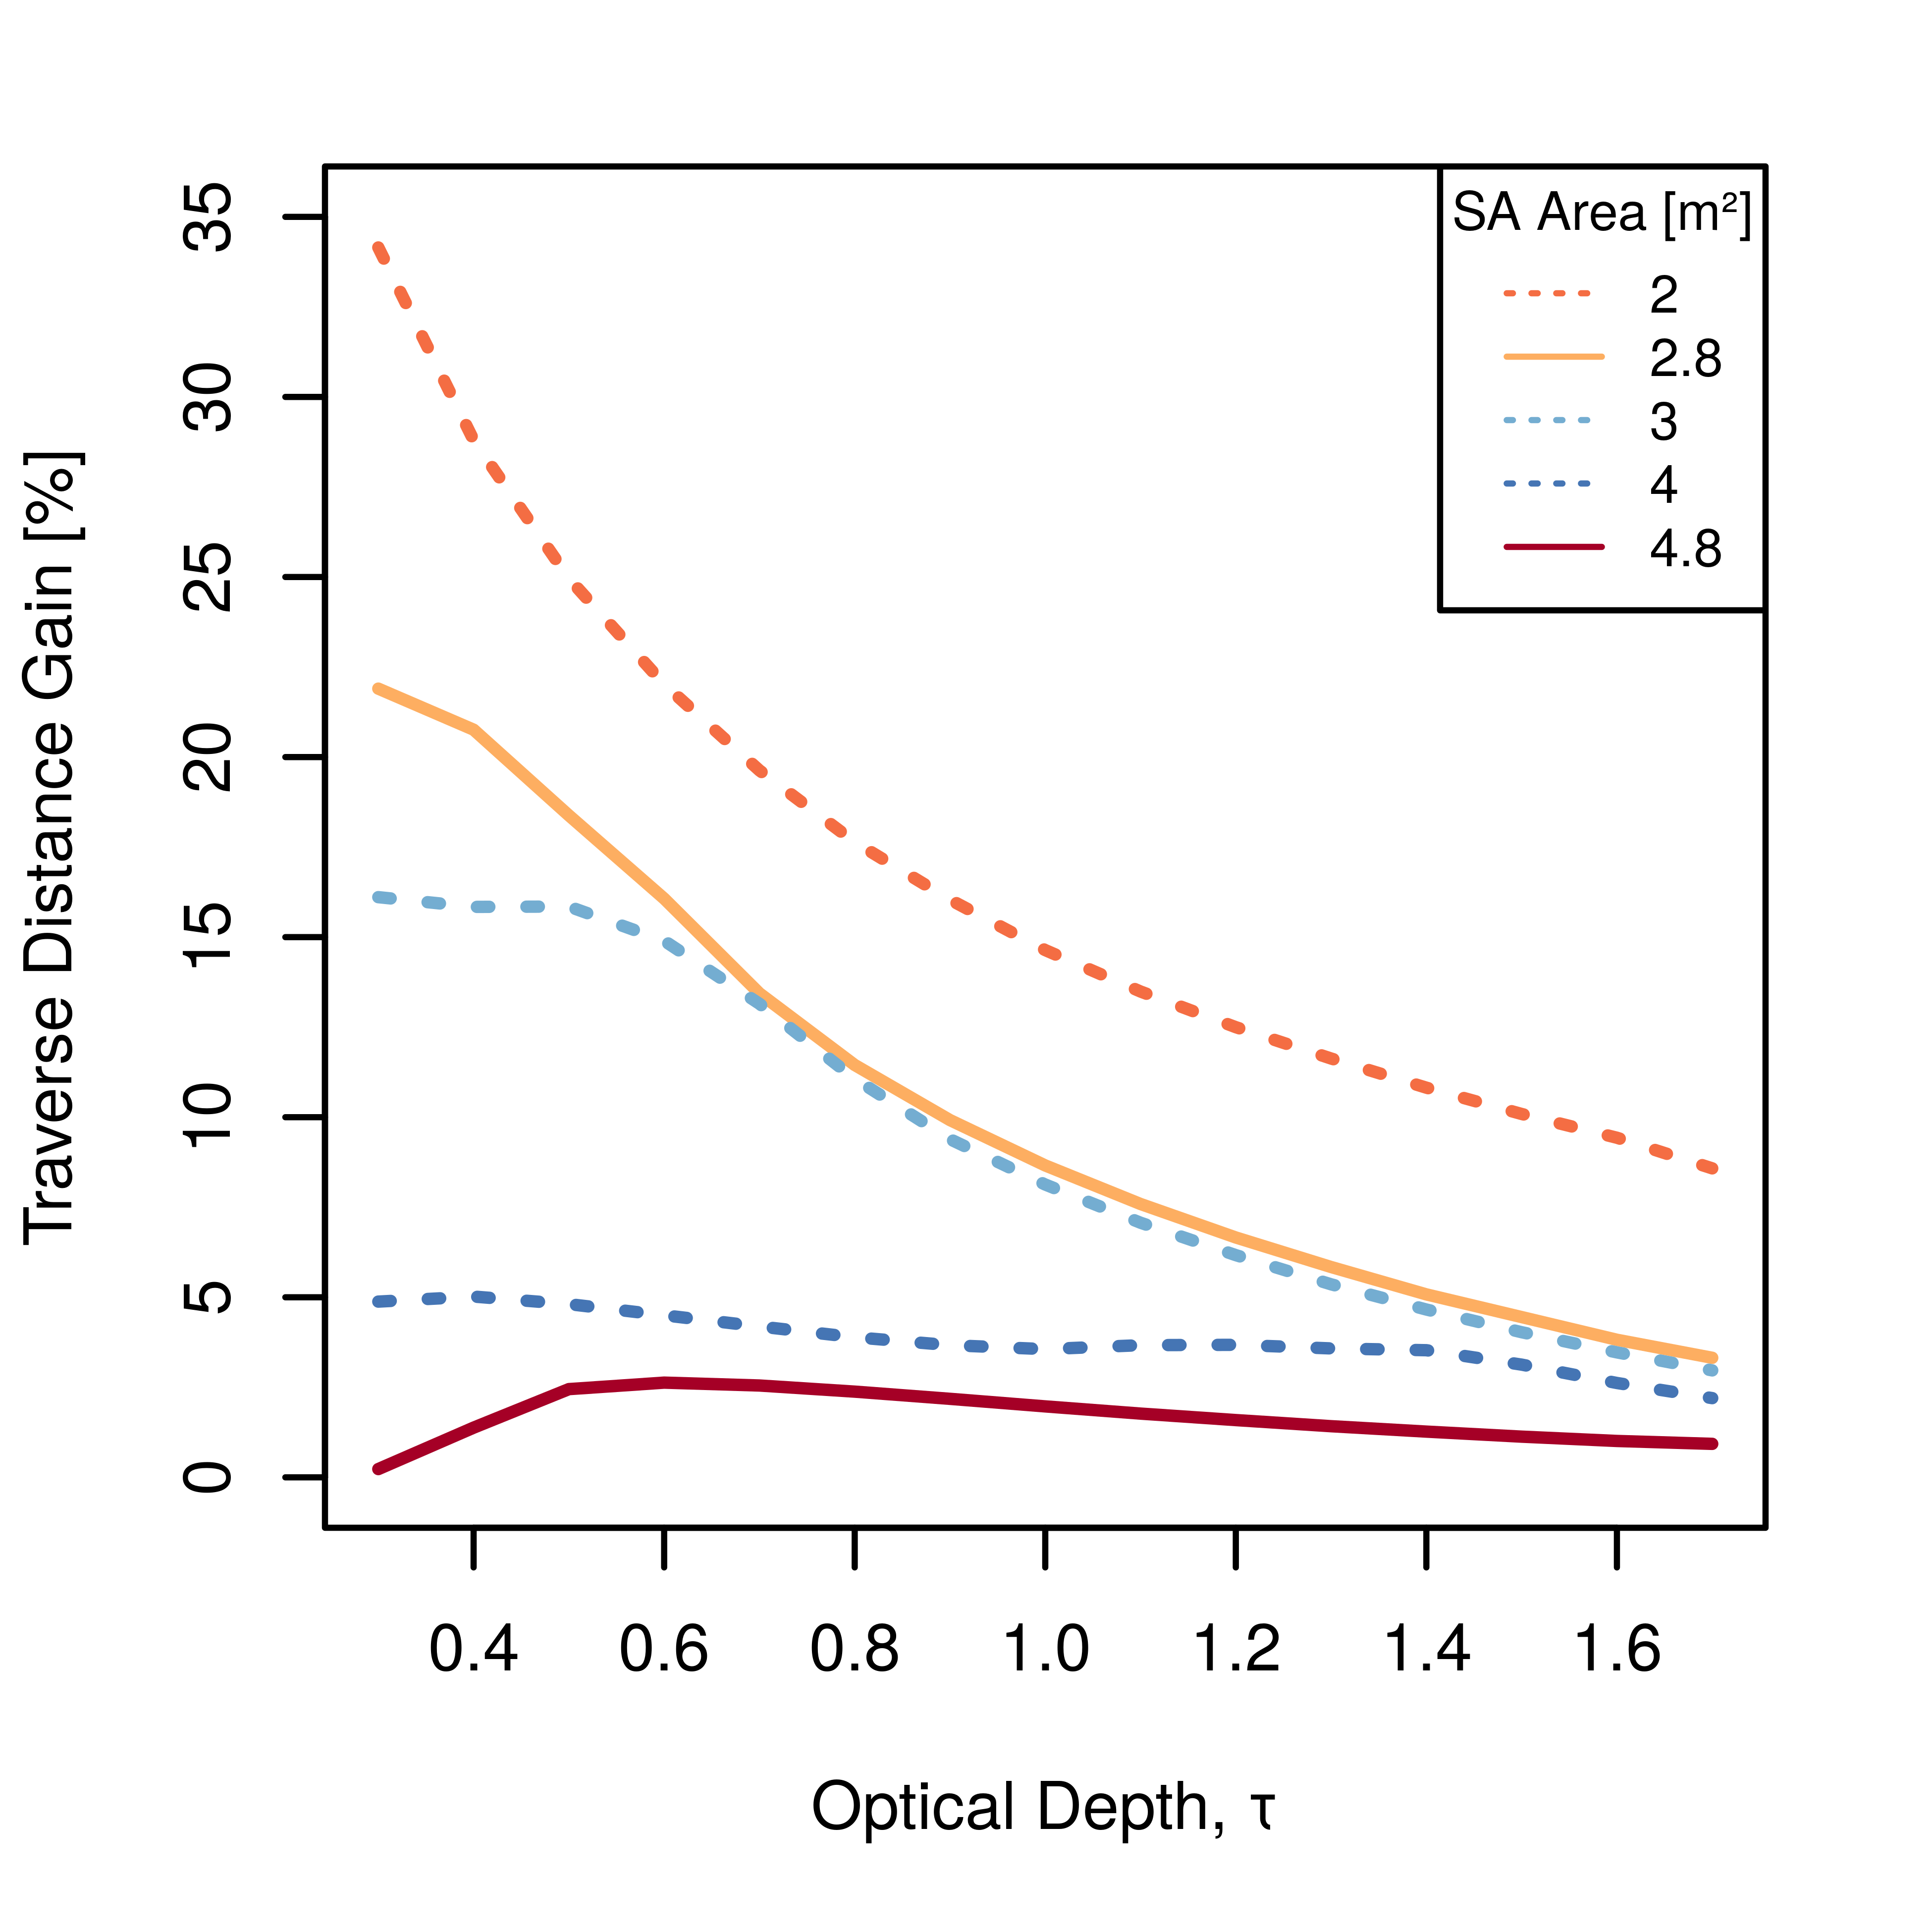
\includegraphics[height=\graphicsHeight]{sections/design/solar-array/plots/ismeniuscavus-75w-traverse-gains-for-different-sa-areas.png}
  		\subcaption{Ismenius Cavus, \ac{SA} area = \SI{2.8}{m^{2}}}
		\label{fig:plot:sub:iani-chaos-flat-traverse-gains-for-different-sa-area}
	\end{subfigure}\\[0.8ex]
    \caption[Flat traverse distance gains at Iani Chaos and Ismenius Cavus for different \ac{SA} sizes]
            {Flat traverse distance gains at Iani Chaos and Ismenius Cavus for different \ac{SA} sizes.}
    \label{fig:plot:flat-traverse-gains-for-different-sa-area}
\vspace{-2ex}
\end{figure}

\begin{figure}[h]
\captionsetup[subfigure]{justification=centering}
\vspace{-2ex}
	\centering
    %% setup sizes
    \setlength{\subfigureWidth}{0.50\textwidth}
    \setlength{\graphicsHeight}{80mm}
    %% kill hyper-link highlighting
    \hypersetup{hidelinks=true}%
    %% the figures
    \begin{subfigure}[t]{\subfigureWidth}
        \centering
        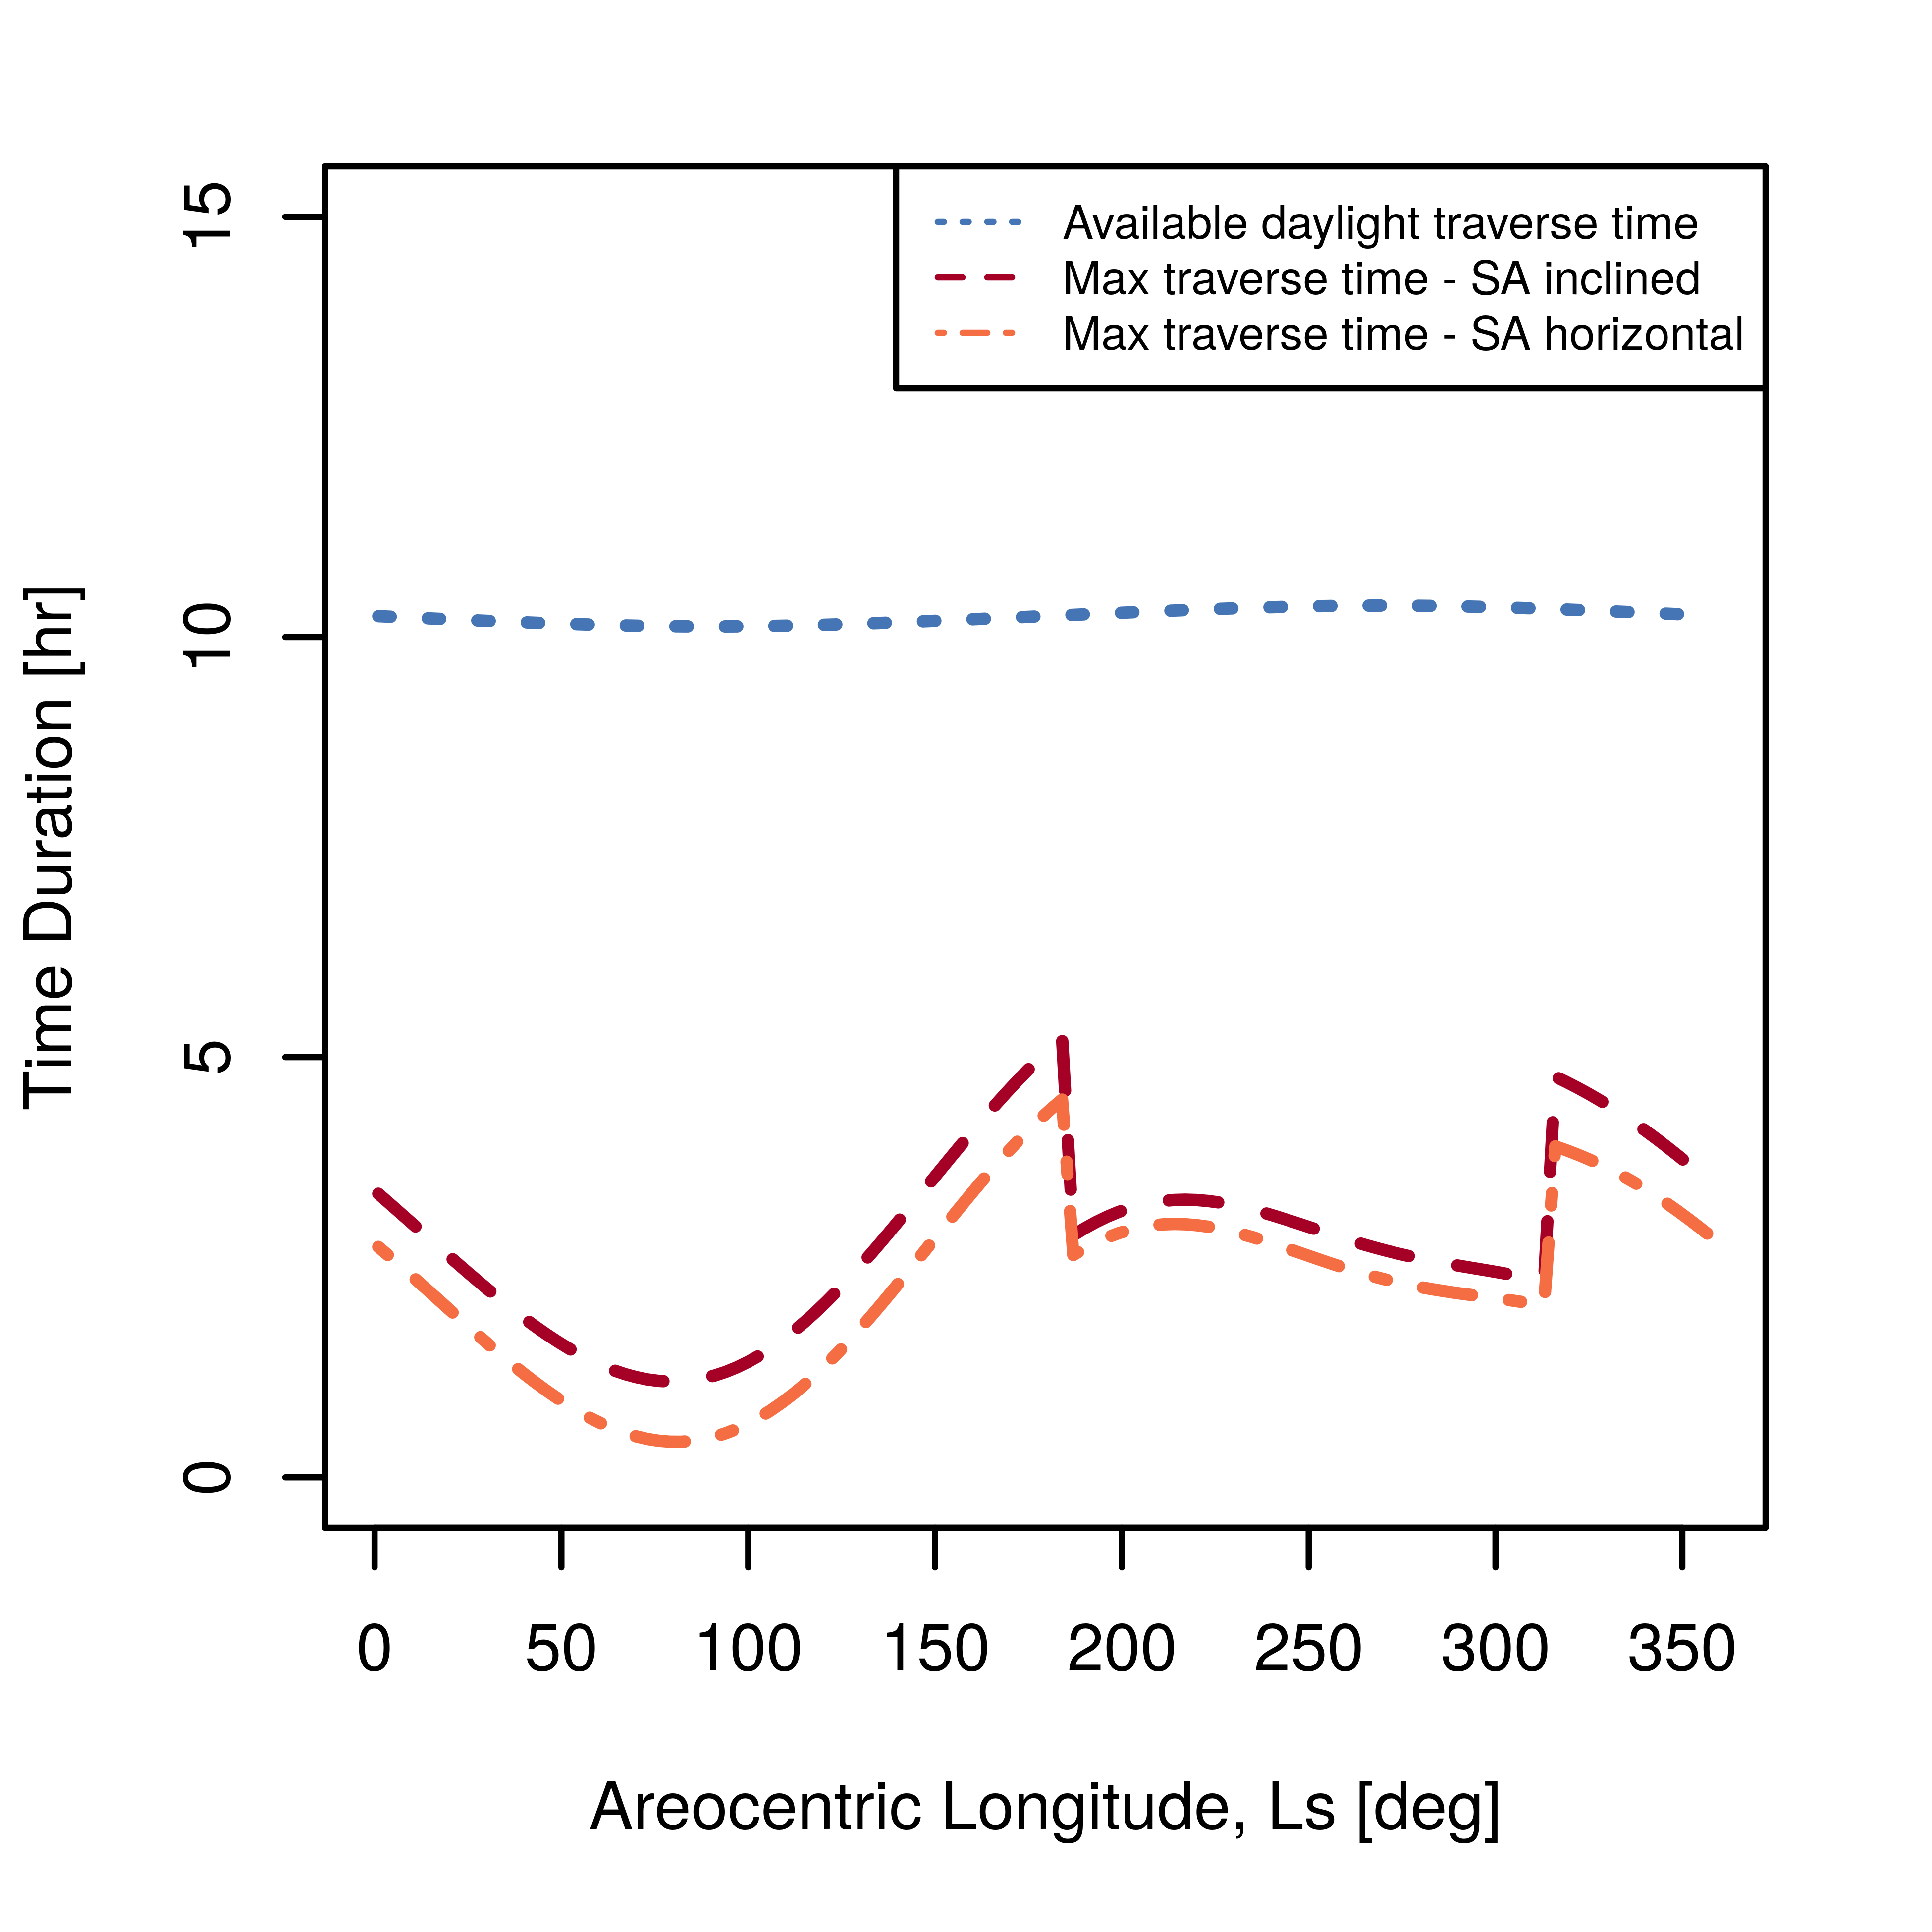
\includegraphics[height=\graphicsHeight]{sections/design/solar-array/plots/ianichaos-75w-max-traverse-durations-for-sa-area-17m2.png}
  		\subcaption{Iani Chaos, \ac{SA} area = \SI{1.7}{m^{2}}}
		\label{fig:plot:sub:final-maximum-traverse-durations-iani-chaos}
    \end{subfigure}\hfill
    \begin{subfigure}[t]{\subfigureWidth}
        \centering
        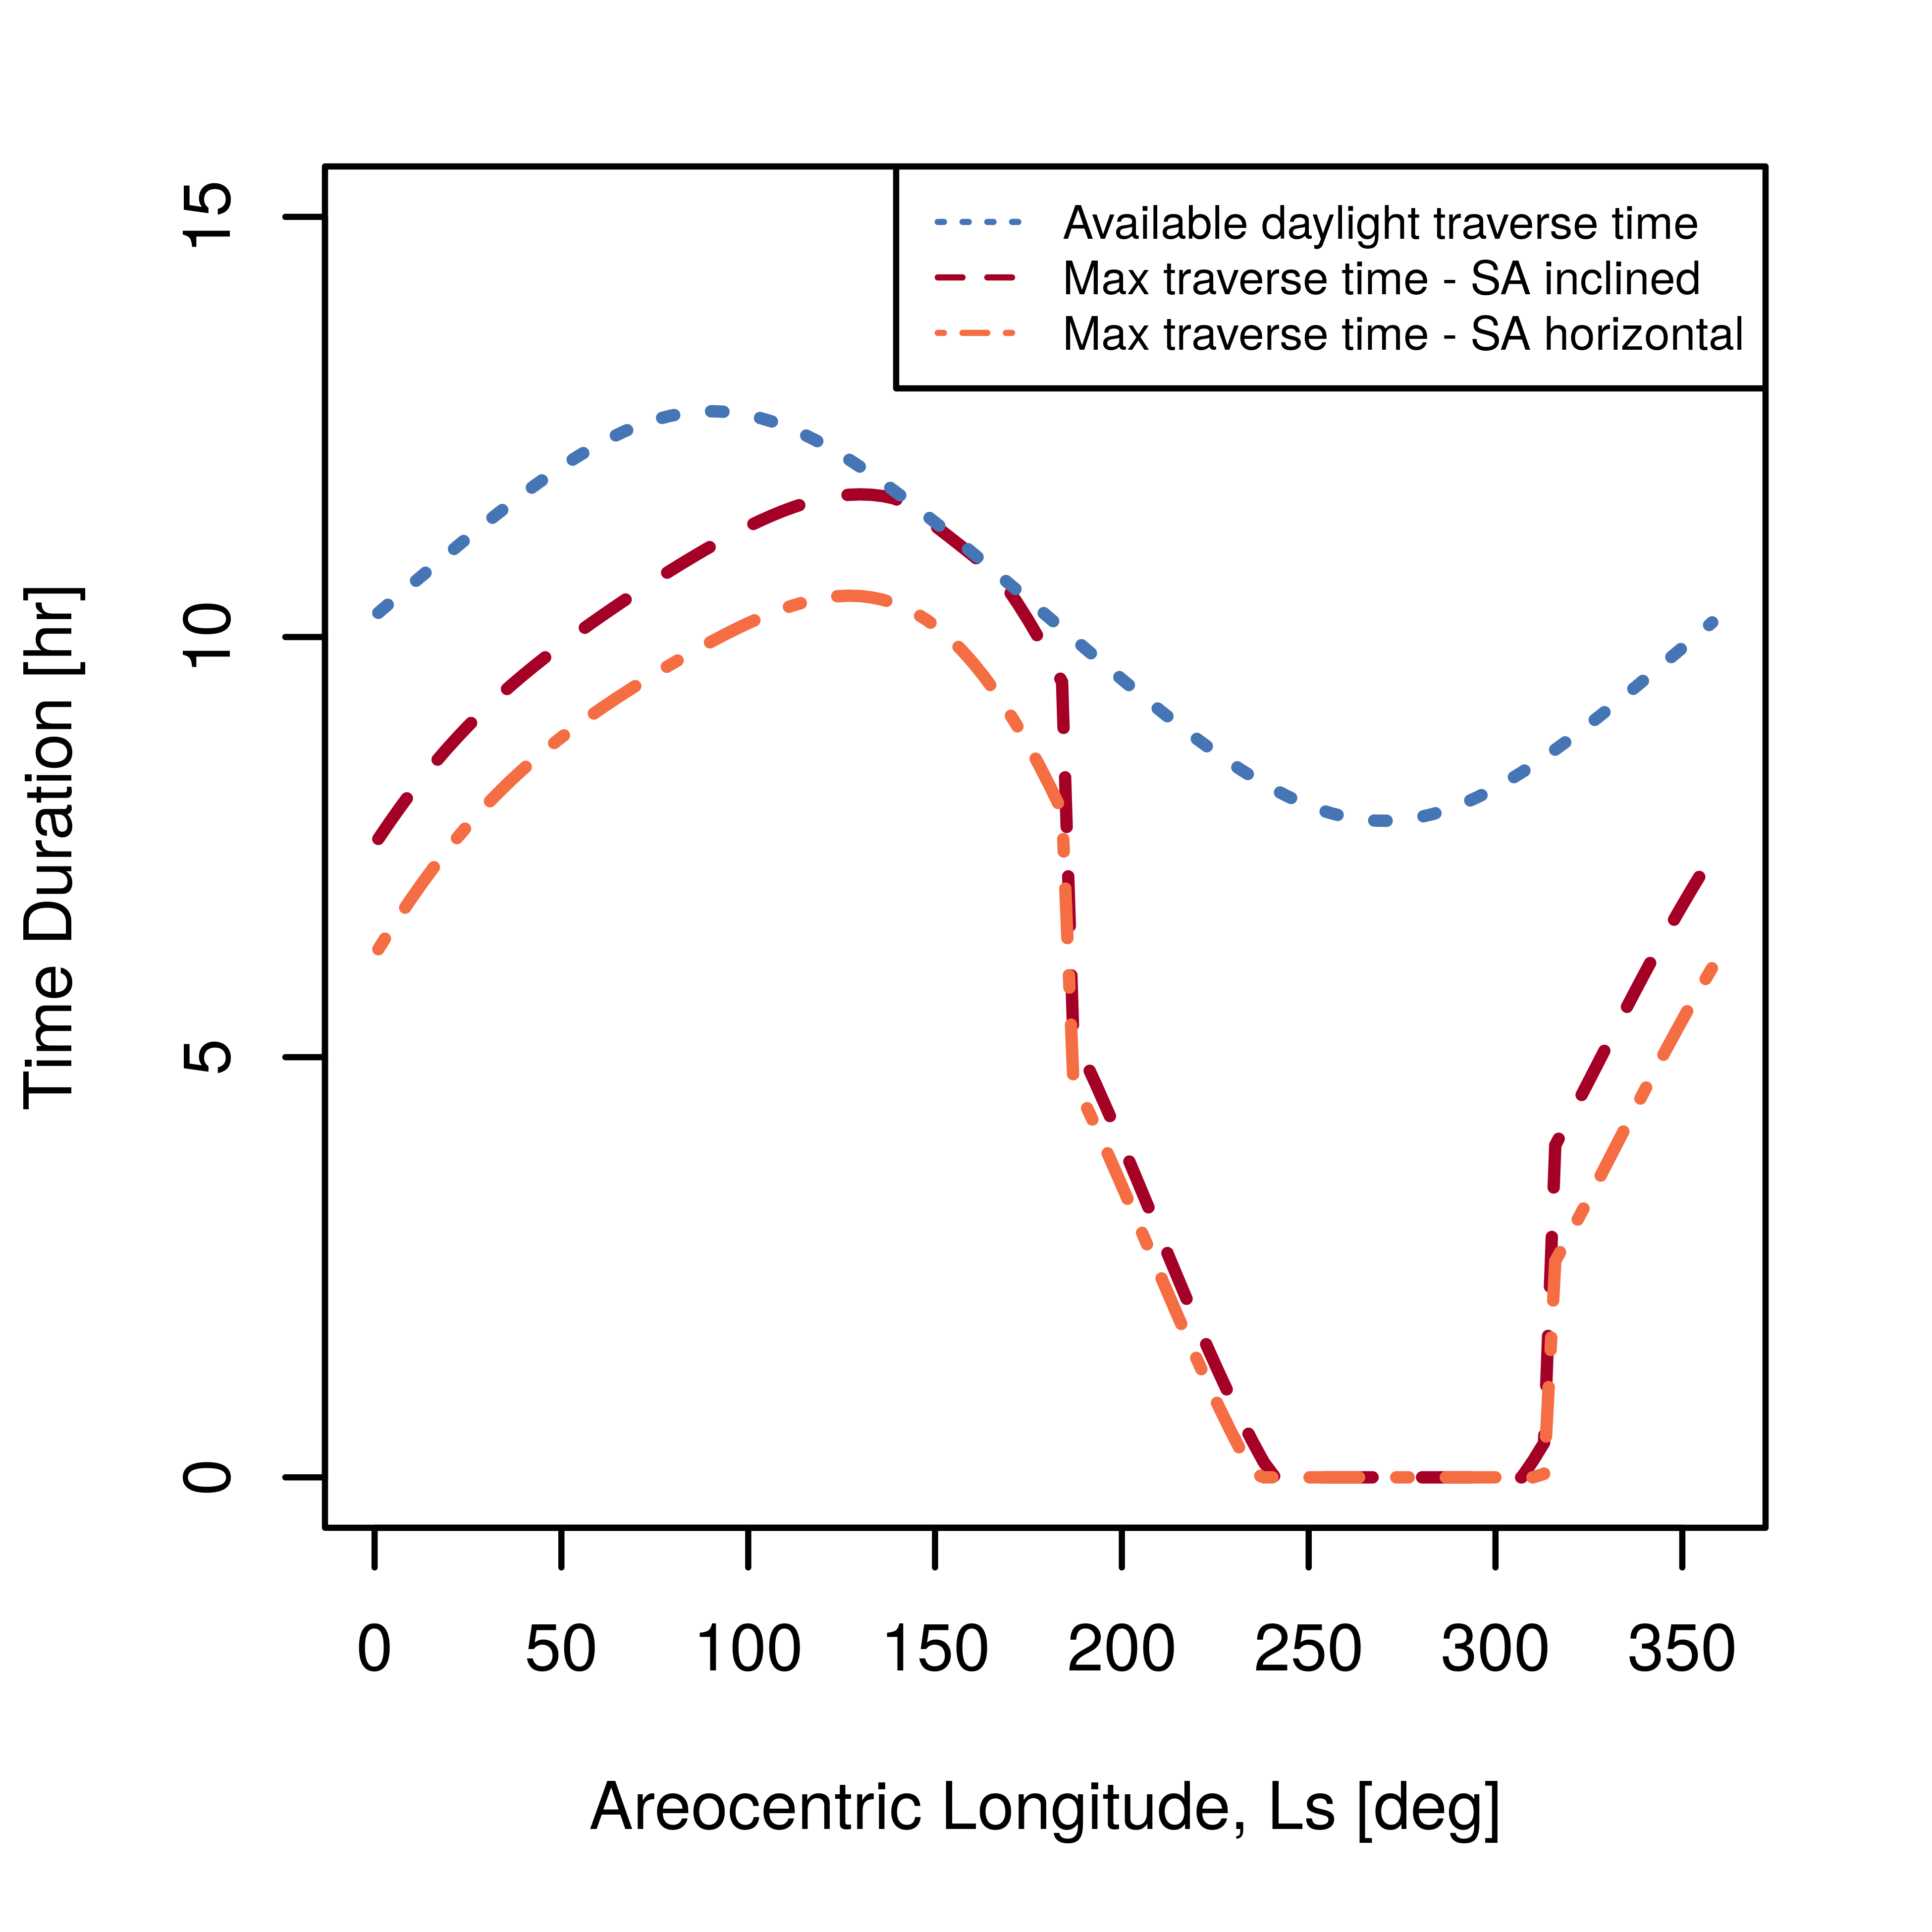
\includegraphics[height=\graphicsHeight]{sections/design/solar-array/plots/ismeniuscavus-75w-max-traverse-durations-for-sa-area-28m2.png}
  		\subcaption{Ismenius Cavus, \ac{SA} area = \SI{2.8}{m^{2}}}
		\label{fig:plot:sub:final-maximum-traverse-durations-ismenius-cavus}
	\end{subfigure}\\[0.8ex]
    \caption[Maximum traverse durations at Iani Chaos and Ismenius Cavus]
            {Maximum traverse durations at Iani Chaos and Ismenius Cavus.}
    \label{fig:plot:final-maximum-traverse-durations-at-missions-sites}
\vspace{-2ex}
\end{figure}


%\clearpage
%\subsubsection{Battery}
%\todo[inline]{\textbf{TODO:} Battery size based on energy required to keep the rover Warm through the night. Check if the calculated size satisfies the hibernation requirement. If not, resize.}

\clearpage
\subsection{Baseline Design}
As per \ref{itm:dd:shadowing}, the rover's body is redesigned in order to minimize shadowing events. A pyramid shaped body continuously casts a shadow on a surrounding \ac{SA} with an exception during solar noon. Even then, it is likely that the rover would be tilted to achieve $\beta_{best}$ and thus still be subject to shadowing. The redesigned body shown in Figure \ref{fig:rover-body-redesign} opts for a box shape with a flat top on which one of the \ac{SA} panels can be placed. The dimension of the redesigned body is $\SI{65}{\centi\meter}\times\SI{65}{\centi\meter}\times\SI{63}{\centi\meter}$ with the base preserving the pyramid body's dimension in order to minimize changes in sizing dependent considerations.

\begin{figure}[h]
\captionsetup[subfigure]{justification=centering}
\vspace{-2ex}
	\centering
    %% setup sizes
    \setlength{\subfigureWidth}{0.50\textwidth}
    \setlength{\graphicsHeight}{48mm}
    %% kill hyper-link highlighting
    \hypersetup{hidelinks=true}%
    %% the figures
    \begin{subfigure}[t]{\subfigureWidth}
        \centering
        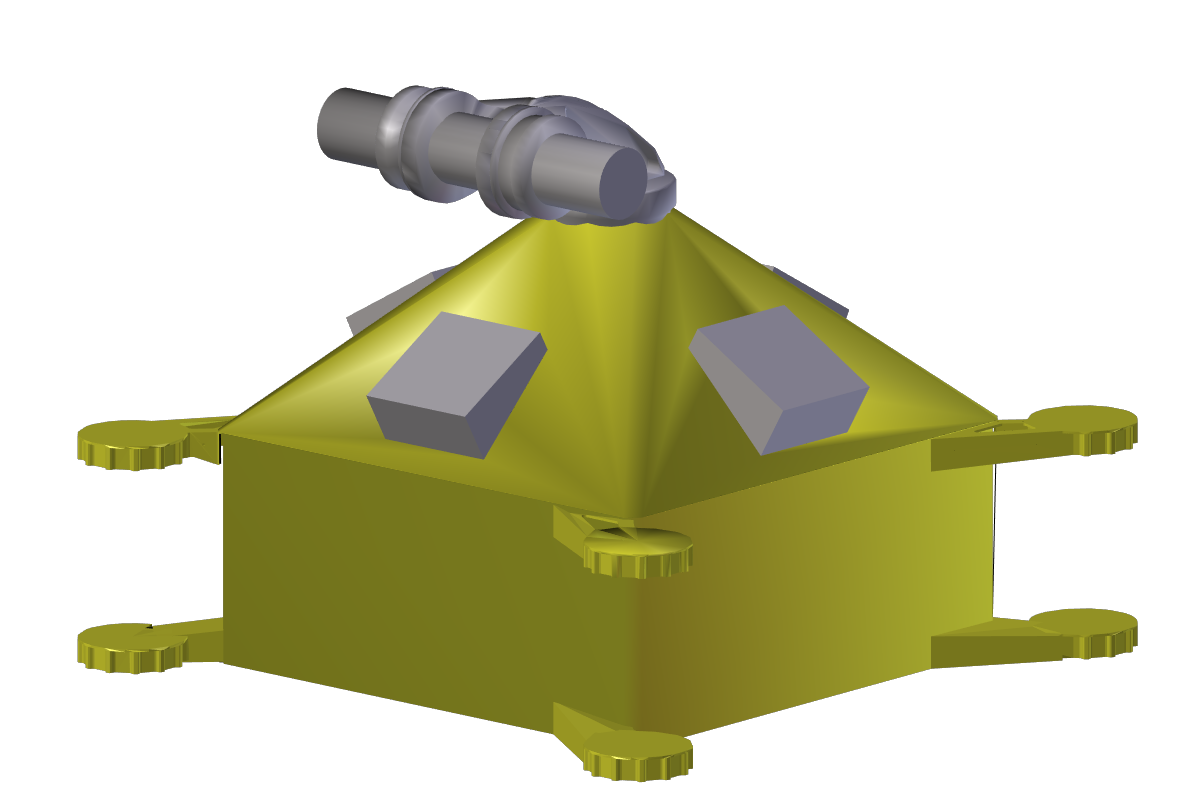
\includegraphics[height=\graphicsHeight]{sections/design/solar-array/images/body-before.png}
        \subcaption{Before}
		\label{fig:sub:rover-body-redesign-before}
    \end{subfigure}\hfill
    \begin{subfigure}[t]{\subfigureWidth}
        \centering
        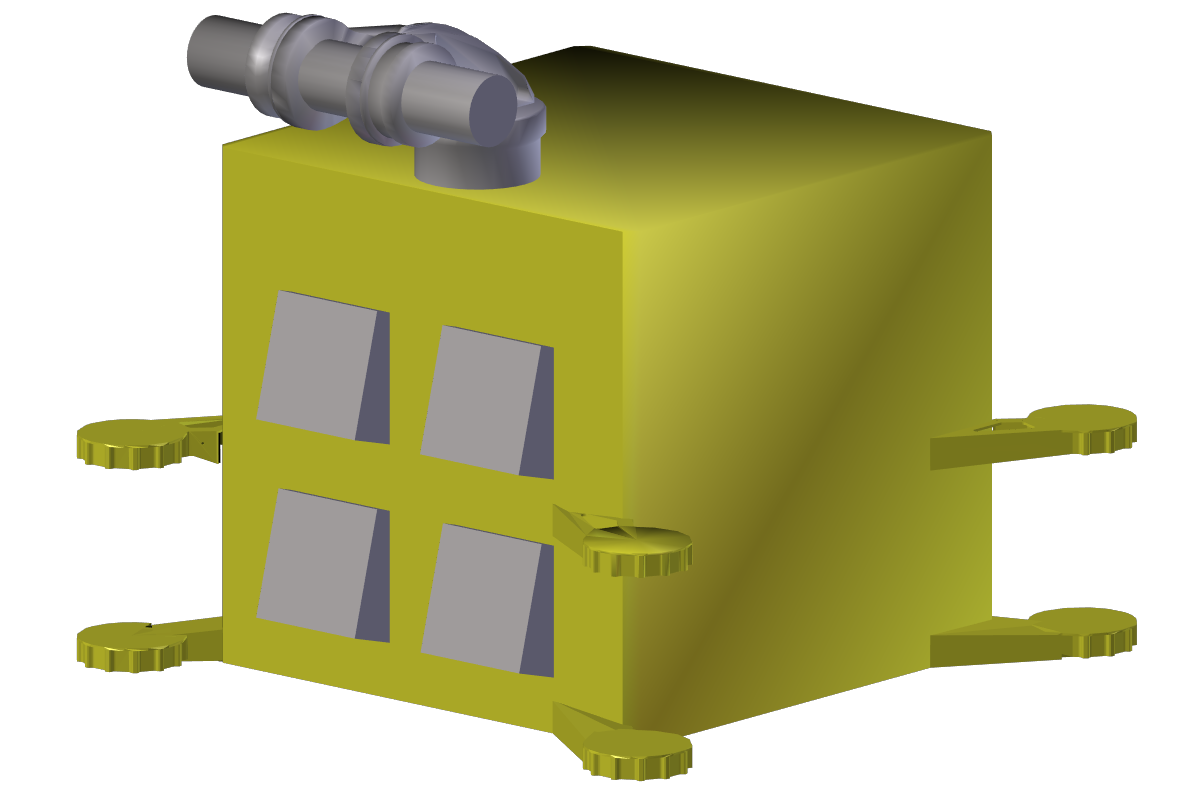
\includegraphics[height=\graphicsHeight]{sections/design/solar-array/images/body-after.png}
  		\subcaption{After}
		\label{fig:sub:rover-body-redesign-after}
	\end{subfigure}\\[0.8ex]
    \caption[Rover body redesign]
            {Rover body redesign.}
    \label{fig:rover-body-redesign}
\vspace{-2ex}
\end{figure}

Placing the four \acp{PLI} is driven by \ref{itm:dd:four_plis} and shown in Figure \ref{fig:sub:rover-body-redesign-after}. They are stored in the front of body and are accessible by the rover's robotic arm. As will be seen further in this section, access to the remaining faces is obstructed by the \ac{SA} panels. Spacing is left between the \acp{PLI} and the top of the body to allow for instruments. The \acp{PLI} are oriented upwords by \SI{15}{\degree} in order to compensate against possible forward tilts driven by the rover repositioning itself to attain $\beta_{best}$. The upward tilt of the \ac{PLI} have the added benefit of facilitating access to the robotic arm. The position of the latter is shifted towards the front in order to maximize the surface area that can be uninterruptedly covered by solar cells. As per \ref{itm:dd:unobstructed}, the movemement range of the suspension system must remain unobstructed. The height of the redesigned body is such that the deployed \ac{SA} panels are kept above the legs for any configuration of the active suspension system. This is demonstrated in Figure \ref{fig:rover-body-redesign-stowed-legs} where the rover's stowed posture results in its knees reaching their highest point.

\begin{figure}[h]
\captionsetup[subfigure]{justification=centering}
\vspace{-2ex}
	\centering
    %% setup sizes
    \setlength{\subfigureWidth}{0.50\textwidth}
    \setlength{\graphicsHeight}{50mm}
    %% kill hyper-link highlighting
    \hypersetup{hidelinks=true}%
    %% the figures
    \begin{subfigure}[t]{\subfigureWidth}
        \centering
        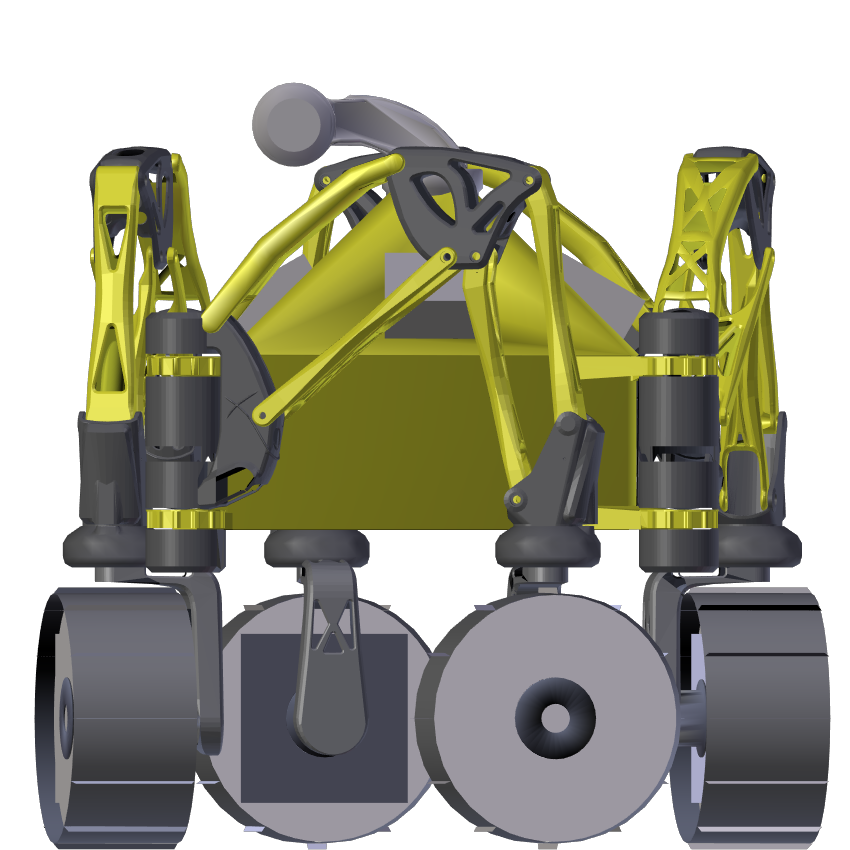
\includegraphics[height=\graphicsHeight]{sections/design/solar-array/images/stowed-body-pyramid.png}
        \subcaption{Before}
		\label{fig:sub:rover-body-redesign-stowed-before}
    \end{subfigure}\hfill
    \begin{subfigure}[t]{\subfigureWidth}
        \centering
        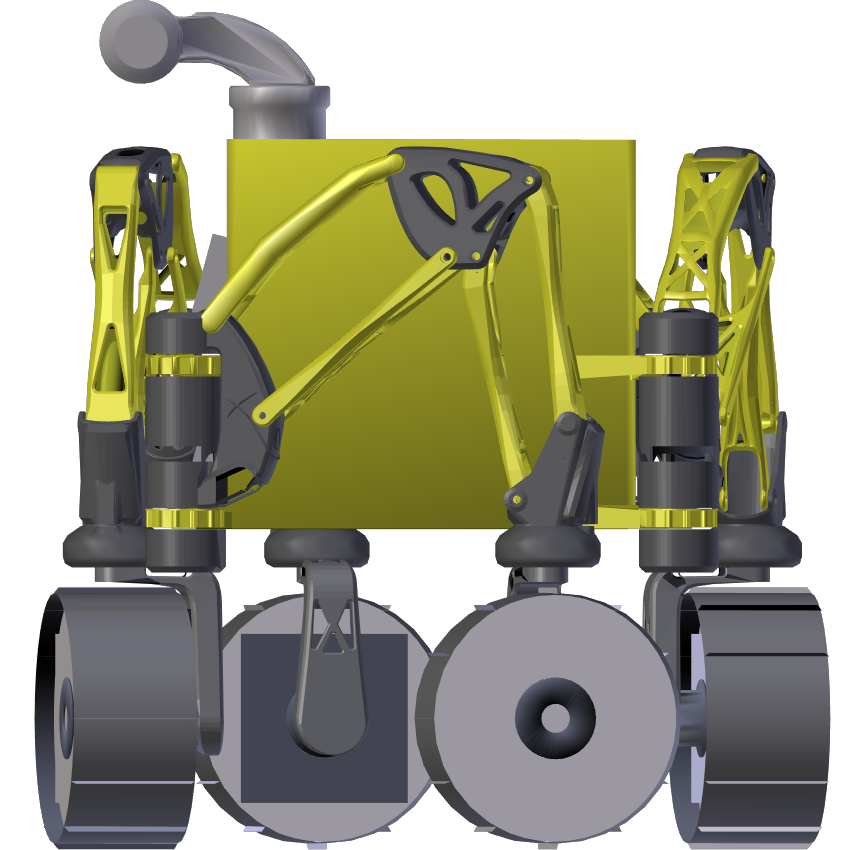
\includegraphics[height=\graphicsHeight]{sections/design/solar-array/images/stowed-body-box.png}
  		\subcaption{After}
		\label{fig:sub:rover-body-redesign-stowed-legs-after}
	\end{subfigure}\\[0.8ex]
    \caption[Rover body redesign with stowed legs]
            {Rover body redesign with stowed legs.}
    \label{fig:rover-body-redesign-stowed-legs}
\vspace{-2ex}
\end{figure}


Folded and deployed \ac{SA} panels are show in Figures \ref{fig:solar-array-on-rover-iani-chaos} and \ref{fig:solar-array-on-ismenius-cavus-chaos} as they would appear mounted on top of the rover's body for different mission sites. When folded, the port, starboard, and stern panels do not lay on top of the rover's body and are instead kept upright at a \SI{90}{\degree} angle. The base of the robotic arm occupies an area of the body's surface that prevents the panels from folding in completely. Shifting the robotic arm onto its own support in front of the body would resolve this but prevent the rover's front right leg from assuming its stowed position.

\vspace{0.5cm}

\begin{figure}[h]
\captionsetup[subfigure]{justification=centering}
\vspace{-2ex}
	\centering
    %% setup sizes
    \setlength{\subfigureWidth}{0.50\textwidth}
    \setlength{\graphicsHeight}{53mm}
    %% kill hyper-link highlighting
    \hypersetup{hidelinks=true}%
    %% the figures
    \begin{subfigure}[t]{\subfigureWidth}
        \centering
        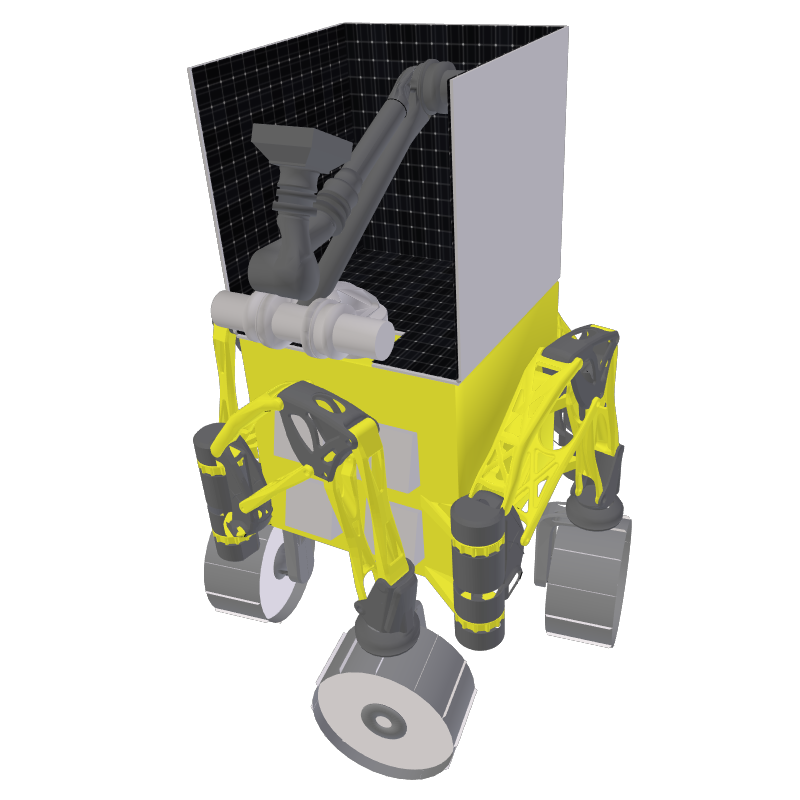
\includegraphics[height=\graphicsHeight]{sections/design/solar-array/images/iani-chaos-stowed.png}
  		\subcaption{Folded on stowed rover}
		\label{fig:sub:solar-array-on-rover-for-iani-chaos-stowed}
    \end{subfigure}\hfill
    \begin{subfigure}[t]{\subfigureWidth}
        \centering
        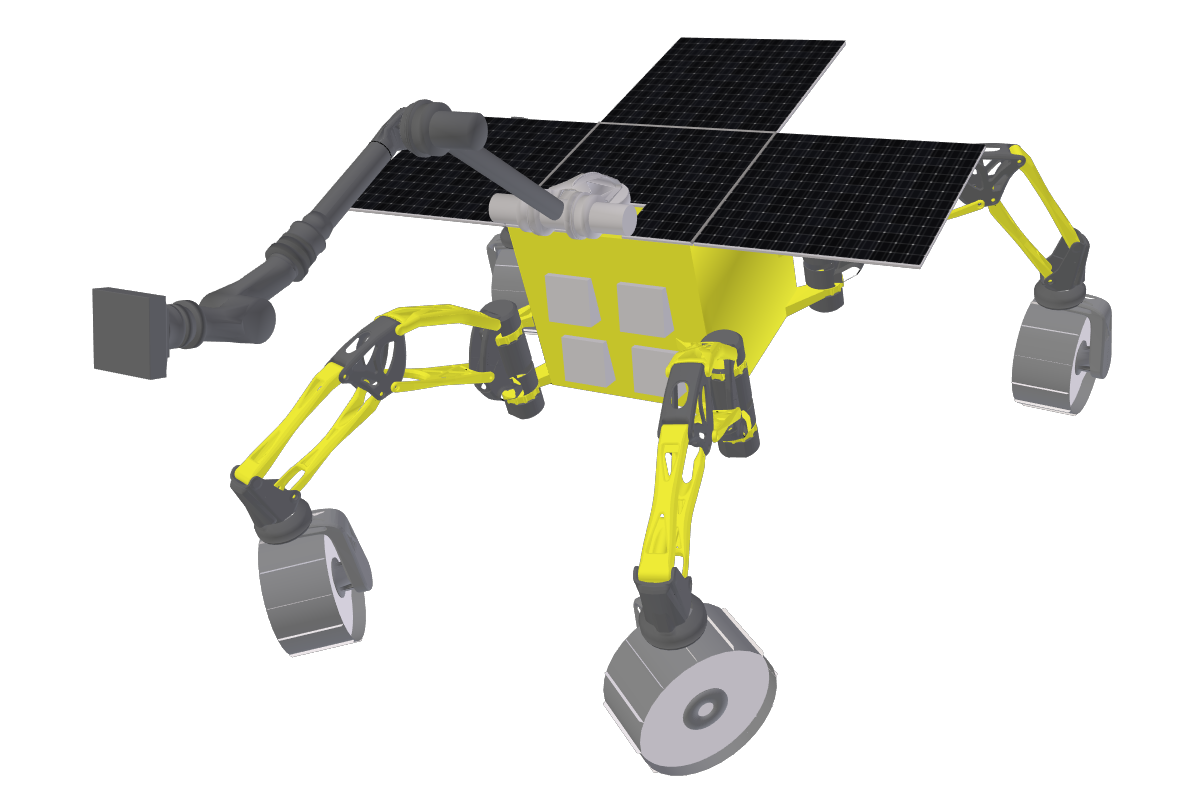
\includegraphics[height=\graphicsHeight]{sections/design/solar-array/images/iani-chaos-10deg-pitch.png}
  		\subcaption{Deployed on rover with \SI{10}{\degree} pitch forward}
		\label{fig:sub:solar-array-on-rover-for-iani-chaos-deployed}
	\end{subfigure}\\[0.8ex]
    \caption[Solar array on rover for Iani Chaos deployment]
            {\ac{SA} on rover for Iani Chaos deployment.}
    \label{fig:solar-array-on-rover-iani-chaos}
\vspace{-2ex}
\end{figure}

\vspace{0.5cm}

The folded configurations shown in Figures \ref{fig:sub:solar-array-on-rover-for-iani-chaos-stowed} and \ref{fig:sub:solar-array-on-rover-for-iani-chaos-deployed} were accepted considering that the gain in height does not add much to what is already imposed by the stowed robotic arm. In terms of compactness, a preferable configuration would be one in which all panels are folded in and the robotic arm is stowed against the front side of the body. However, supporting existing rover postures is preferred within the scope of this work. Future design iterations of the stowed configuration for both the robotic arm and the \ac{SA} panels should prioritize compactness based on a \ac{LV} payload capacity and the rover's lander constraints.

\vspace{0.5cm}

\begin{figure}[h]
\captionsetup[subfigure]{justification=centering}
\vspace{-2ex}
	\centering
    %% setup sizes
    \setlength{\subfigureWidth}{0.50\textwidth}
    \setlength{\graphicsHeight}{53mm}
    %% kill hyper-link highlighting
    \hypersetup{hidelinks=true}%
    %% the figures
    \begin{subfigure}[t]{\subfigureWidth}
        \centering
        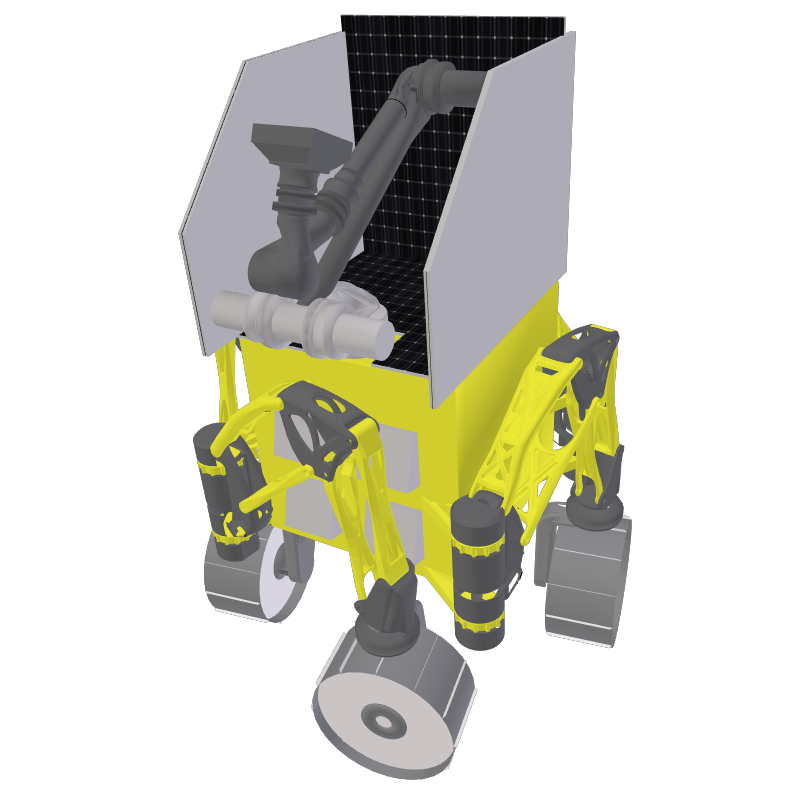
\includegraphics[height=\graphicsHeight]{sections/design/solar-array/images/ismenius-cavus-stowed.png}
  		\subcaption{Folded on stowed rover}
		\label{fig:sub:solar-array-on-rover-for-ismenius-cavus-stowed}
    \end{subfigure}\hfill
    \begin{subfigure}[t]{\subfigureWidth}
        \centering
        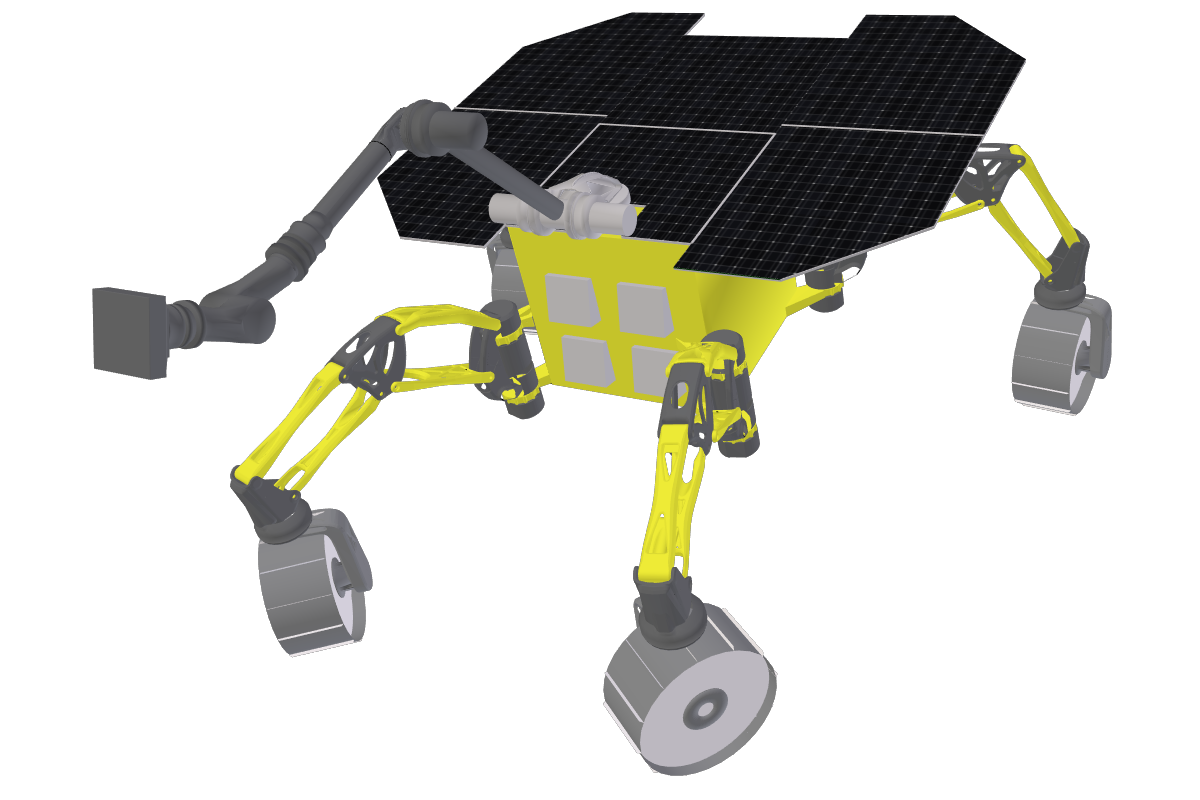
\includegraphics[height=\graphicsHeight]{sections/design/solar-array/images/ismenius-cavus-10deg-pitch.png}
  		\subcaption{Deployed on rover with \SI{10}{\degree} pitch forward}
		\label{fig:sub:solar-array-on-rover-for-ismenius-cavus-deployed}
	\end{subfigure}\\[0.8ex]
    \caption[Solar array on rover for Ismenius Cavus deployment]
            {\ac{SA} on rover for Ismenius Cavus deployment.}
    \label{fig:solar-array-on-ismenius-cavus-chaos}
\vspace{-2ex}
\end{figure}

\clearpage
The unfolded \ac{SA} panel layouts are shown in Figure \ref{fig:solar-array-layouts-for-missions-sites}. The \ac{SA} at Iani Chaos consists of four panels whereas a six panel design is used at Ismenius Cavus. The bow panels require a cut to accomodate the base of the rover's robotic arm.

\vspace{0.5cm}

\begin{figure}[h]
\captionsetup[subfigure]{justification=centering}
\vspace{-2ex}
	\centering
    %% setup sizes
    \setlength{\subfigureWidth}{0.50\textwidth}
    \setlength{\graphicsHeight}{53mm}
    %% kill hyper-link highlighting
    \hypersetup{hidelinks=true}%
    %% the figures
    \begin{subfigure}[t]{\subfigureWidth}
        \centering
        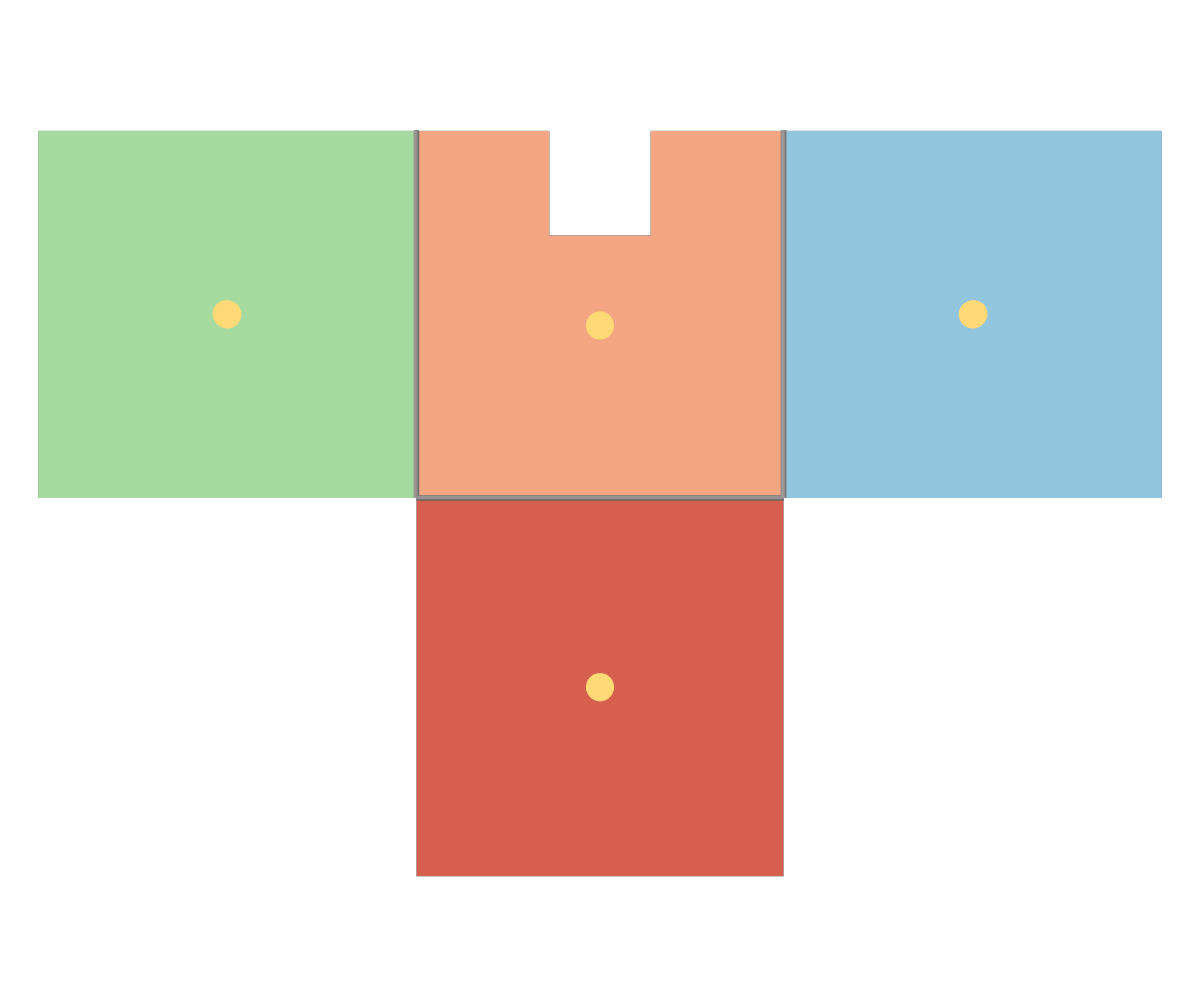
\includegraphics[height=\graphicsHeight]{sections/design/solar-array/images/solar_array_layout_iani_chaos.png}
  		\subcaption{Iani Chaos, \ac{SA} area = \SI{1.7}{m^{2}}}
		\label{fig:sub:solar-array-layouts-for-iani-chaos}
    \end{subfigure}\hfill
    \begin{subfigure}[t]{\subfigureWidth}
        \centering
        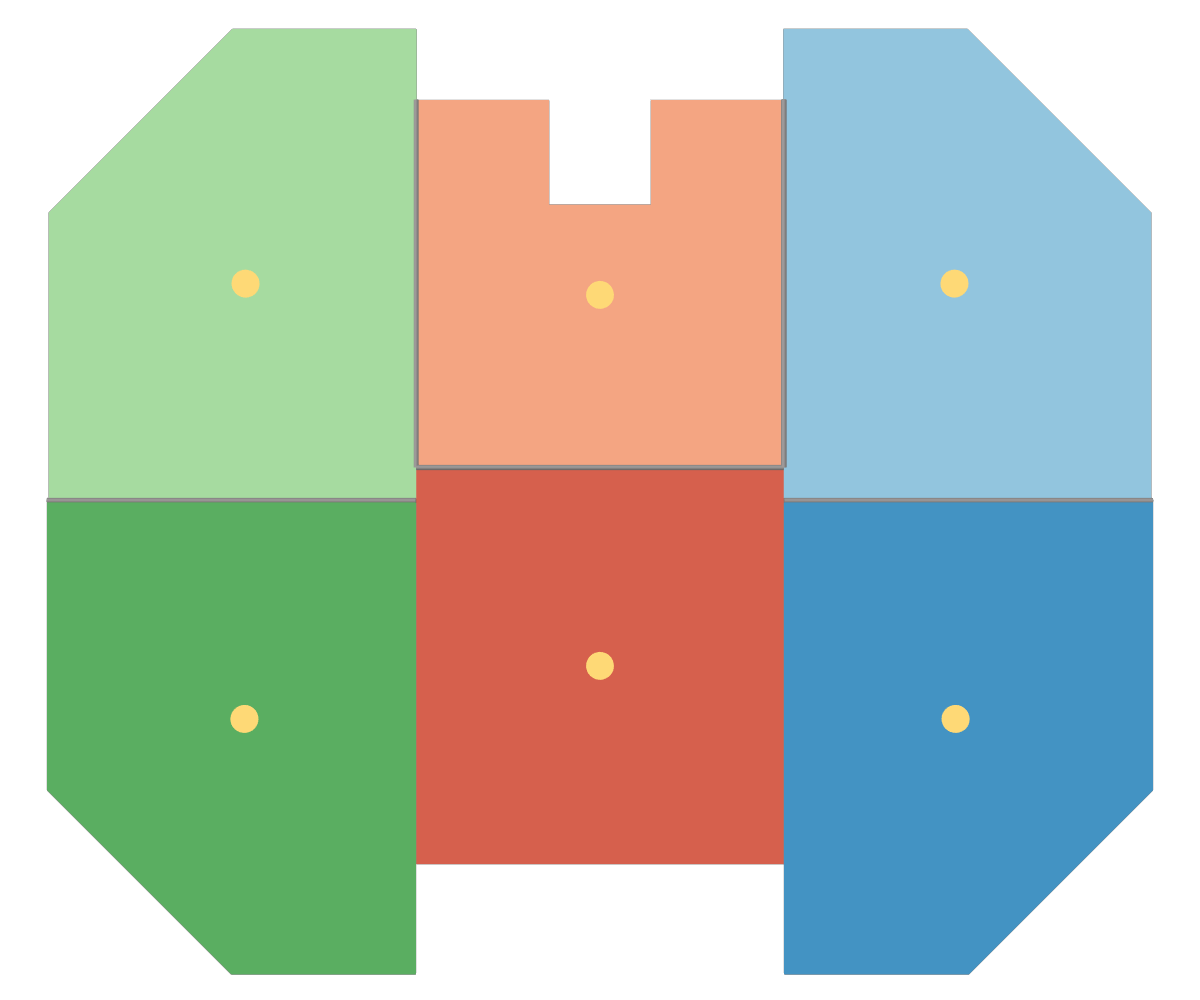
\includegraphics[height=\graphicsHeight]{sections/design/solar-array/images/solar_array_layout_ismenius_cavus.png}
  		\subcaption{Ismenius Cavus, \ac{SA} area = \SI{2.8}{m^{2}}}
		\label{fig:sub:solar-array-layouts-for-ismenius-cavus}
	\end{subfigure}\\[0.8ex]
    \caption[Solar array layouts]
            {\ac{SA} layouts. Green and blue panels are located on the rover's port and starboard, respectively. Port bow and stardboard bow panels are indicated by lighter colors than those on the rover's port quarter and starboard quarter. Light red indicates bow panels which rest over the rover's body. Darker red panels are located on the rover's stern. The yellow dots represent the \ac{CoM} for each panel.}
    \label{fig:solar-array-layouts-for-missions-sites}
\vspace{-2ex}
\end{figure}

\vspace{0.5cm}

Round and diagonal edges negatively affect solar cell packing efficiency and are thus avoided. However, a trade-off is made at Ismenius Cavus due to the large coverage area of the panels and in light of \ref{itm:dd:cog}. Diagonal corners are used for the port and starboard panels to reduce the wingspan of the solar array while preserving the \ac{CoG} within the stowed rover's body and to reduce the panel \ac{CoM} misalignments when they are deployed. Further \ac{CoG} analysis is required for both configurations with respect to the stern and quarter panels when operating the rover's manipulator arm. This could result in shifting the position of the port and starboard panels. The surface areas and masses of each panel are presented in Table \ref{tab:solar-panel-surface-areas}. Masses were determined from \ref{itm:ass:sa_surface_density} with \ac{SA} surface density of \SI{3.7}{kg.m^{-2}}.

\vspace{0.5cm}

\begin{table}[h]
\footnotesize
\centering
\caption{Solar panel surface areas and mass for mission site solar arrays.}
\label{tab:solar-panel-surface-areas}
\begin{tabular}{l|c|c|c|c|}
\cline{2-5}
\textbf{} & \multicolumn{2}{c|}{\textbf{Iani Chaos}} & \multicolumn{2}{c|}{\textbf{Ismenius Cavus}} \\ \cline{2-5}
 & \textbf{Surface Area {[}m2{]}} & \textbf{Mass {[}kg{]}} & \textbf{Surface Area {[}m2{]}} & \textbf{Mass {[}kg{]}} \\ \hline
\multicolumn{1}{|l|}{{\color[HTML]{A6DBA0} \textbf{Port bow}}} & {\color[HTML]{A6DBA0} \textbf{0.44}} & {\color[HTML]{A6DBA0} \textbf{1.63}} & {\color[HTML]{A6DBA0} \textbf{0.50}} & {\color[HTML]{A6DBA0} \textbf{1.85}} \\ \hline
\multicolumn{1}{|l|}{{\color[HTML]{5AAE61} \textbf{Port quarter}}} & {\color[HTML]{5AAE61} \textbf{-}} & {\color[HTML]{5AAE61} \textbf{-}} & {\color[HTML]{5AAE61} \textbf{0.50}} & {\color[HTML]{5AAE61} \textbf{1.85}} \\ \hline
\multicolumn{1}{|l|}{{\color[HTML]{F4A582} \textbf{Bow}}} & {\color[HTML]{F4A582} \textbf{0.38}} & {\color[HTML]{F4A582} \textbf{1.41}} & {\color[HTML]{F4A582} \textbf{0.38}} & {\color[HTML]{F4A582} \textbf{1.41}} \\ \hline
\multicolumn{1}{|l|}{{\color[HTML]{D6604D} \textbf{Stern}}} & {\color[HTML]{D6604D} \textbf{0.44}} & {\color[HTML]{D6604D} \textbf{1.63}} & {\color[HTML]{D6604D} \textbf{0.42}} & {\color[HTML]{D6604D} \textbf{1.55}} \\ \hline
\multicolumn{1}{|l|}{{\color[HTML]{92C5DE} \textbf{Starboard bow}}} & {\color[HTML]{92C5DE} \textbf{0.44}} & {\color[HTML]{92C5DE} \textbf{1.63}} & {\color[HTML]{92C5DE} \textbf{0.50}} & {\color[HTML]{92C5DE} \textbf{1.85}} \\ \hline
\multicolumn{1}{|l|}{{\color[HTML]{4393C3} \textbf{Starboard quarter}}} & {\color[HTML]{4393C3} \textbf{-}} & {\color[HTML]{4393C3} \textbf{-}} & {\color[HTML]{4393C3} \textbf{0.50}} & {\color[HTML]{4393C3} \textbf{1.85}} \\ \hline
\multicolumn{1}{|r|}{\textbf{Total}} & \textbf{1.7} & \textbf{6.30} & \textbf{2.8} & \textbf{10.36} \\ \hline
\end{tabular}
\end{table}




\clearpage
\subsection{Mechanisms}
Solar panel deployment sequences are presented in this section. The worst case unfolding is identified with respect to panel mass and traveled rotation distance from which initial motor performance requirements are calculated.

\subsubsection{Deployment Sequence}

\ac{SA} panels deployment at Iani Chaos is straightforward and limited two three unfoldings. Port, bow, and starboard panels are deployed simultaneously while the rover is still in its stowed posture. The sequence is illustrated in Figure \ref{fig:deployment-sequence-iani-chaos}.

\vspace{0.5cm}

\begin{figure}[h]
\captionsetup[subfigure]{justification=centering}
\vspace{-2ex}
	\centering
    %% setup sizes
    \setlength{\subfigureWidth}{0.32\textwidth}
    \setlength{\graphicsHeight}{30mm}
    %% kill hyper-link highlighting
    \hypersetup{hidelinks=true}%
    %% the figures
	\begin{subfigure}[t]{\subfigureWidth}
        \centering
		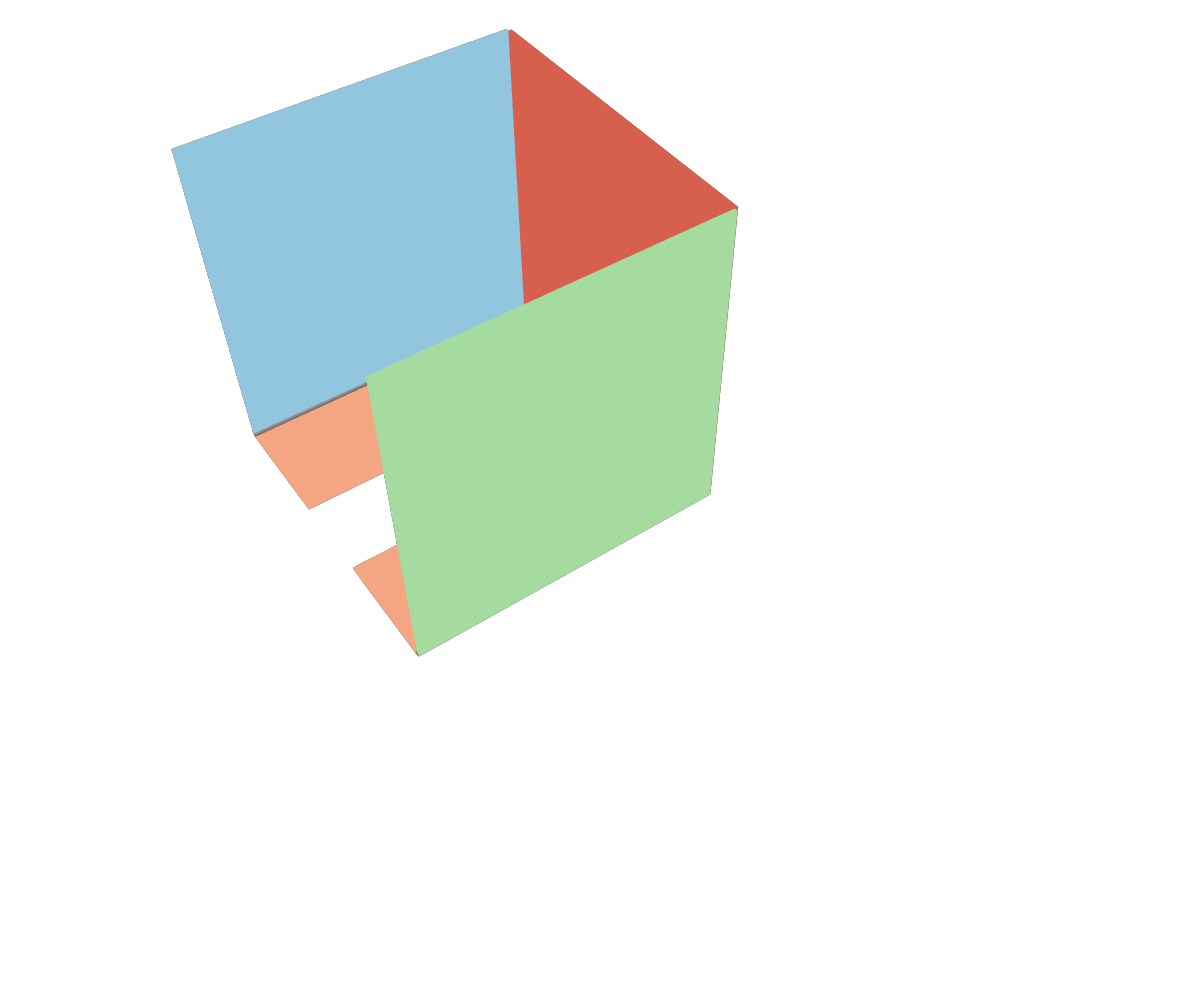
\includegraphics[height=\graphicsHeight]{sections/design/solar-array/images/deployment/iani-chaos/solar_array_deployment_iani_chaos_000.png}
		\subcaption{Folded}
		\label{fig:sub:deployment-sequence-iani-chaos-stowed}
	\end{subfigure}\hfill
	\begin{subfigure}[t]{\subfigureWidth}
        \centering
		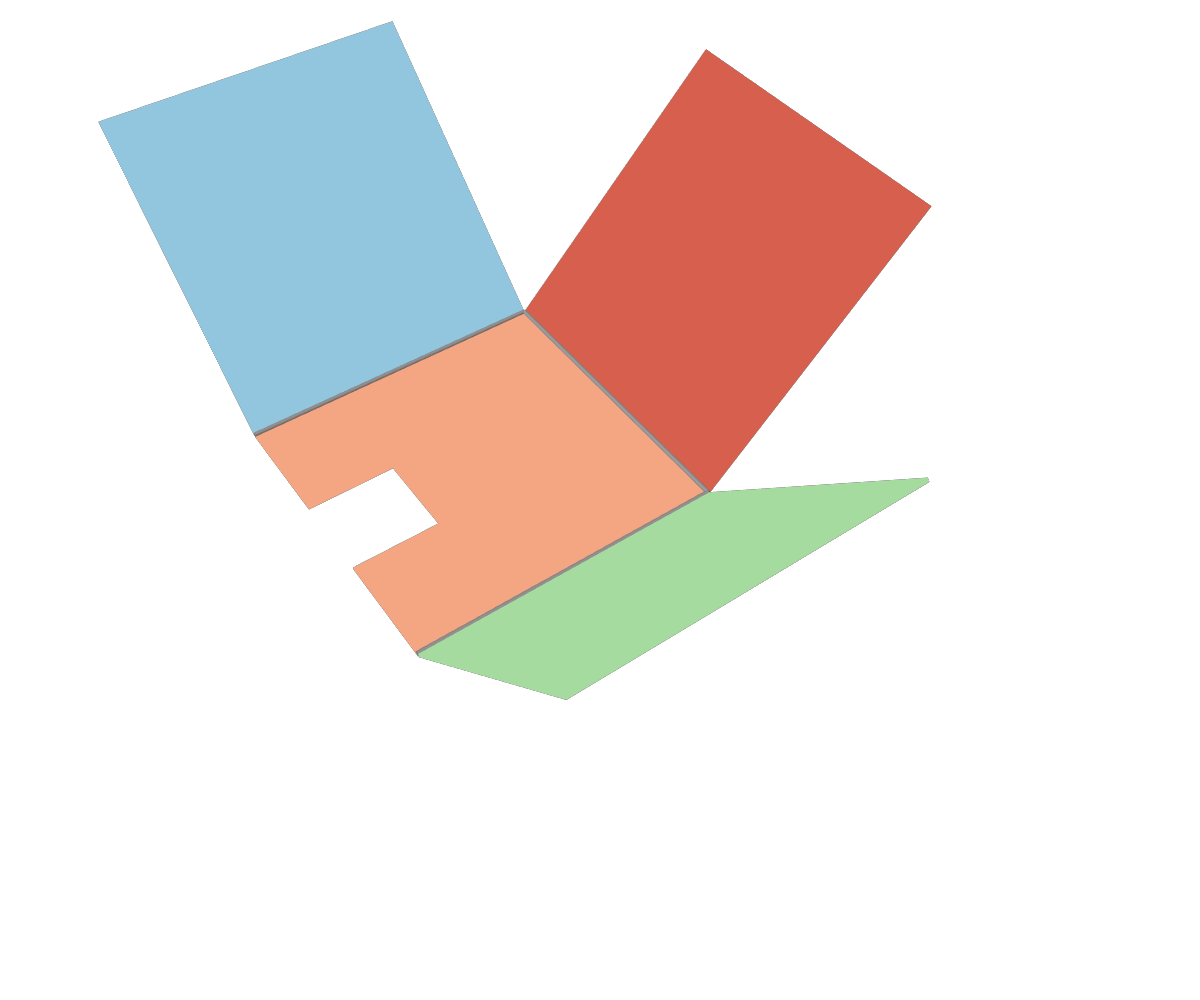
\includegraphics[height=\graphicsHeight]{sections/design/solar-array/images/deployment/iani-chaos/solar_array_deployment_iani_chaos_030.png}
		\subcaption{Mid-deployment}
		\label{fig:sub:deployment-sequence-iani-chaos-mid}
	\end{subfigure}\hfill
    \begin{subfigure}[t]{\subfigureWidth}
        \centering
		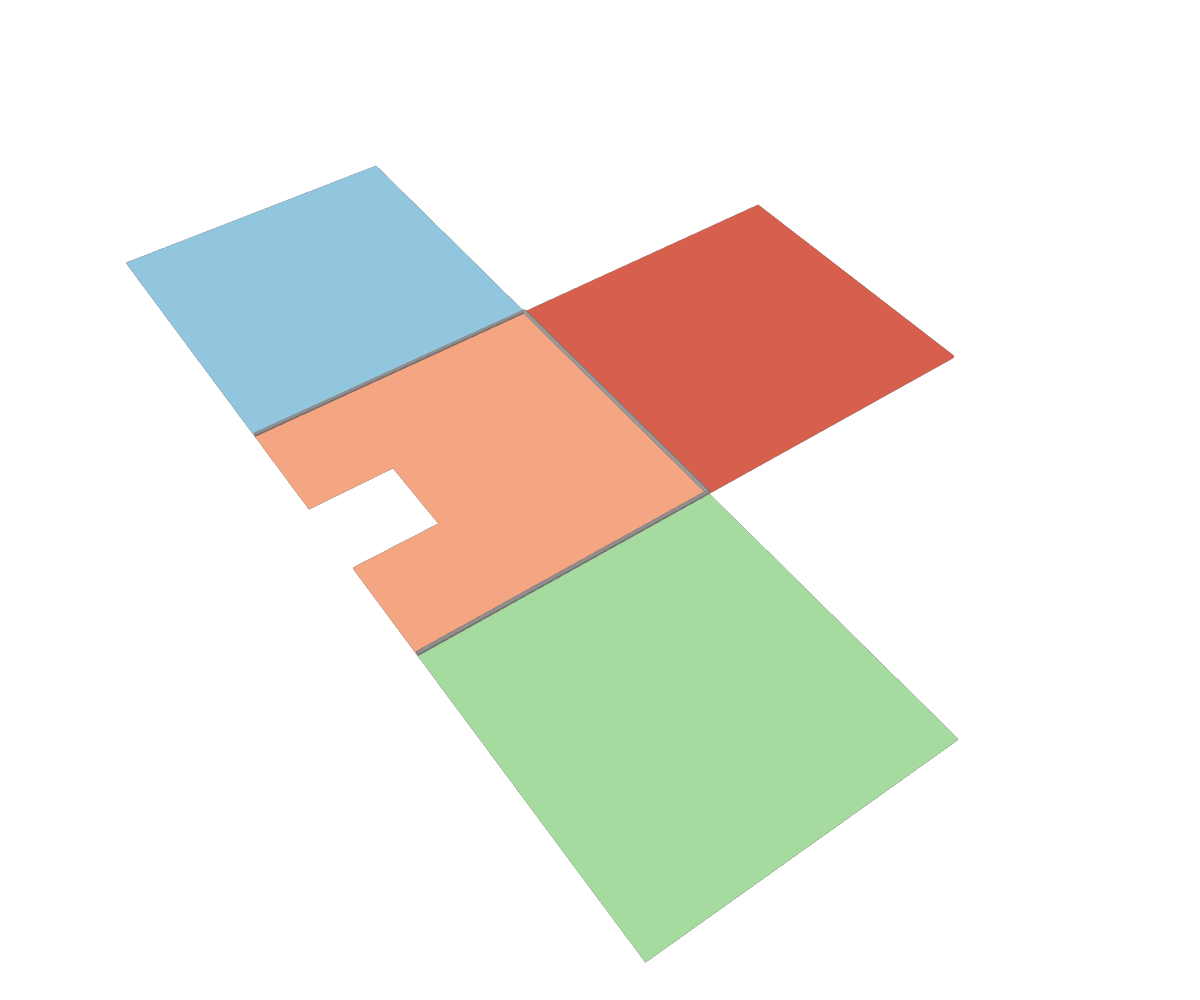
\includegraphics[height=\graphicsHeight]{sections/design/solar-array/images/deployment/iani-chaos/solar_array_deployment_iani_chaos_060.png}
		\subcaption{Deployed}
		\label{fig:sub:deployment-sequence-iani-completed}
	\end{subfigure}
	\caption{Deployment sequence of \SI{1.7}{\meter\squared} solar array at Iani Chaos.}
	\label{fig:deployment-sequence-iani-chaos}
\vspace{-2ex}
\end{figure}

\vspace{0.5cm}

\ac{SA} panels deployment at Ismenius Cavus goes through five unfoldings. The sequence is illustrated in Figure \ref{fig:deployment-sequence-ismenius-cavus}. The port bow, starboard bow, stern panels are simultenously deployed, completing the first three out of the five unfoldings. The remaining two unfoldings deploy the port quarter and starboard quarter panels.

\vspace{0.5cm}

\begin{figure}[h]
\captionsetup[subfigure]{justification=centering}
\vspace{-2ex}
	\centering
    %% setup sizes
    \setlength{\subfigureWidth}{0.32\textwidth}
    \setlength{\graphicsHeight}{30mm}
    %% kill hyper-link highlighting
    \hypersetup{hidelinks=true}%
    %% the figures
	\begin{subfigure}[t]{\subfigureWidth}
        \centering
		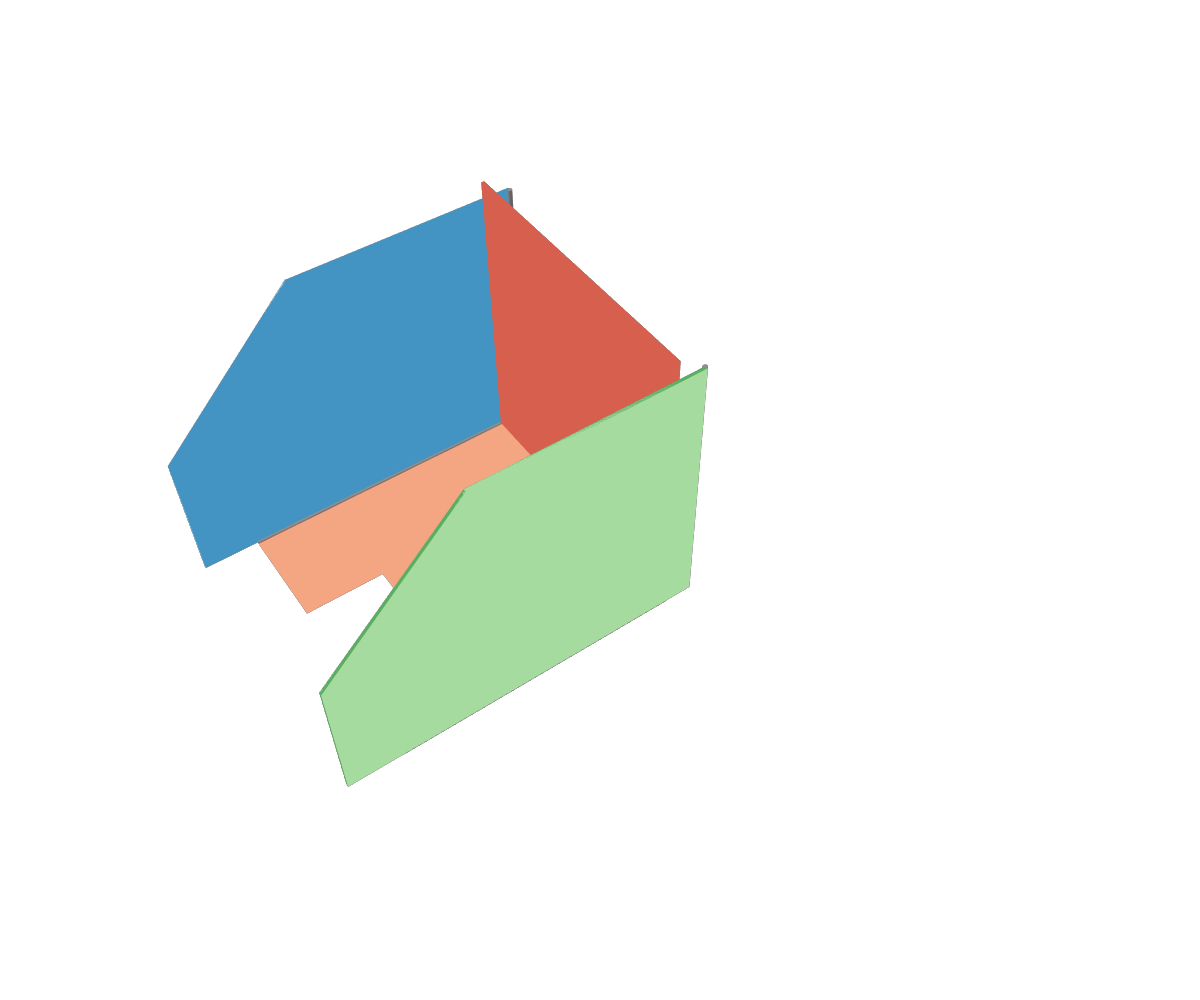
\includegraphics[height=\graphicsHeight]{sections/design/solar-array/images/deployment/ismenius-cavus/solar_array_deployment_ismenius_cavus_000.png}
		\subcaption{Folded panels for stowed posture}
		\label{fig:sub:deployment-sequence-ismenius-cavus-stowed}
	\end{subfigure}\hfill
	\begin{subfigure}[t]{\subfigureWidth}
        \centering
		
\includegraphics[height=\graphicsHeight]{sections/design/solar-array/images/deployment/ismenius-cavus/solar_array_deployment_ismenius_cavus_030.png}
		\subcaption{Port bow, starboard bow, and stern mid-deployment}
		\label{fig:sub:deployment-sequence-ismenius-cavus-mid-bow-and-stern}
	\end{subfigure}\hfill
    \begin{subfigure}[t]{\subfigureWidth}
        \centering
		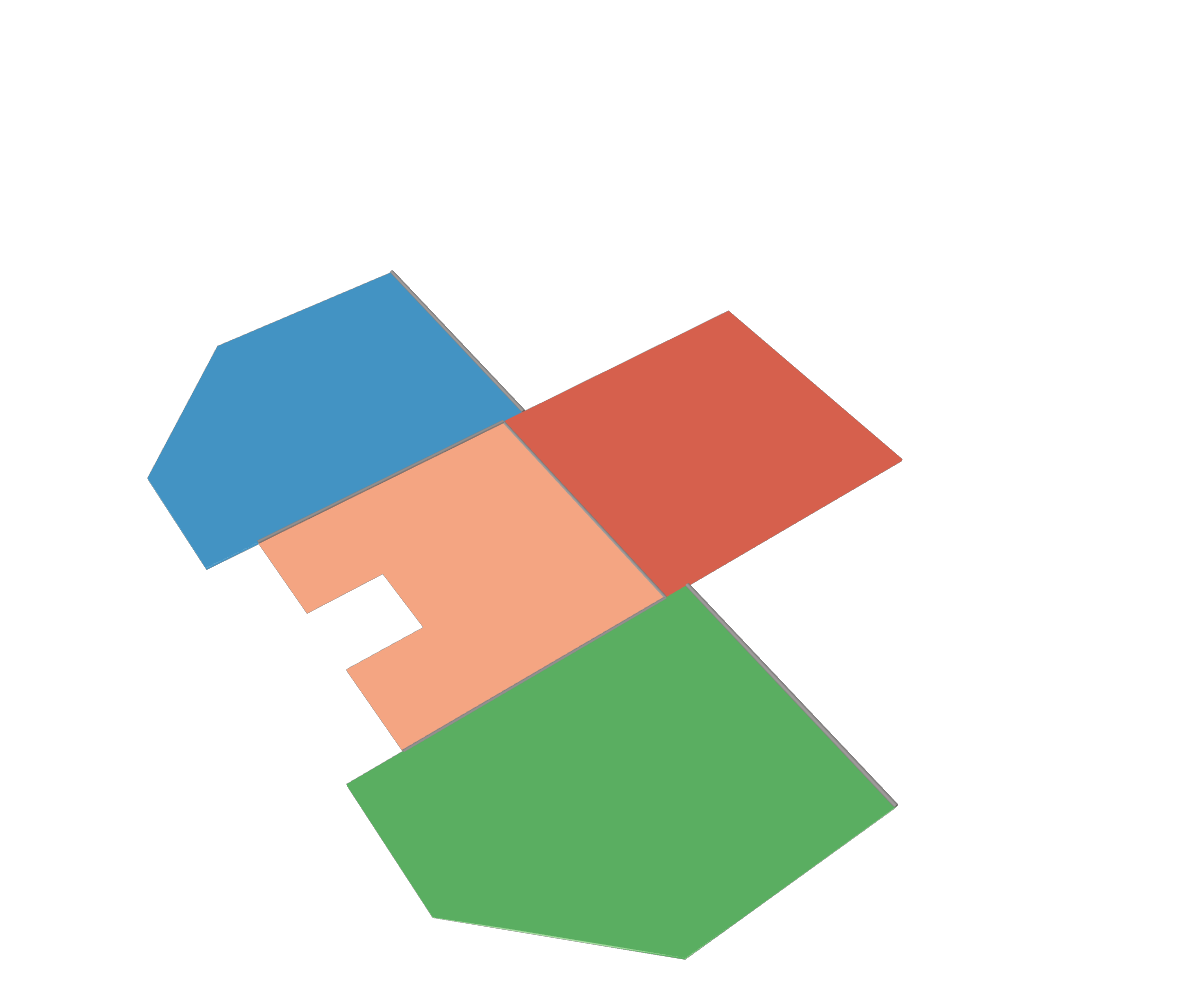
\includegraphics[height=\graphicsHeight]{sections/design/solar-array/images/deployment/ismenius-cavus/solar_array_deployment_ismenius_cavus_060.png}
		\subcaption{Port bow, starboard bow, and stern deployed}
		\label{fig:sub:deployment-sequence-ismenius-cavus-full-bow-and-stern}
	\end{subfigure}\\[0.8ex]
%% 2nd row
	\begin{subfigure}[t]{\subfigureWidth}
        \centering
		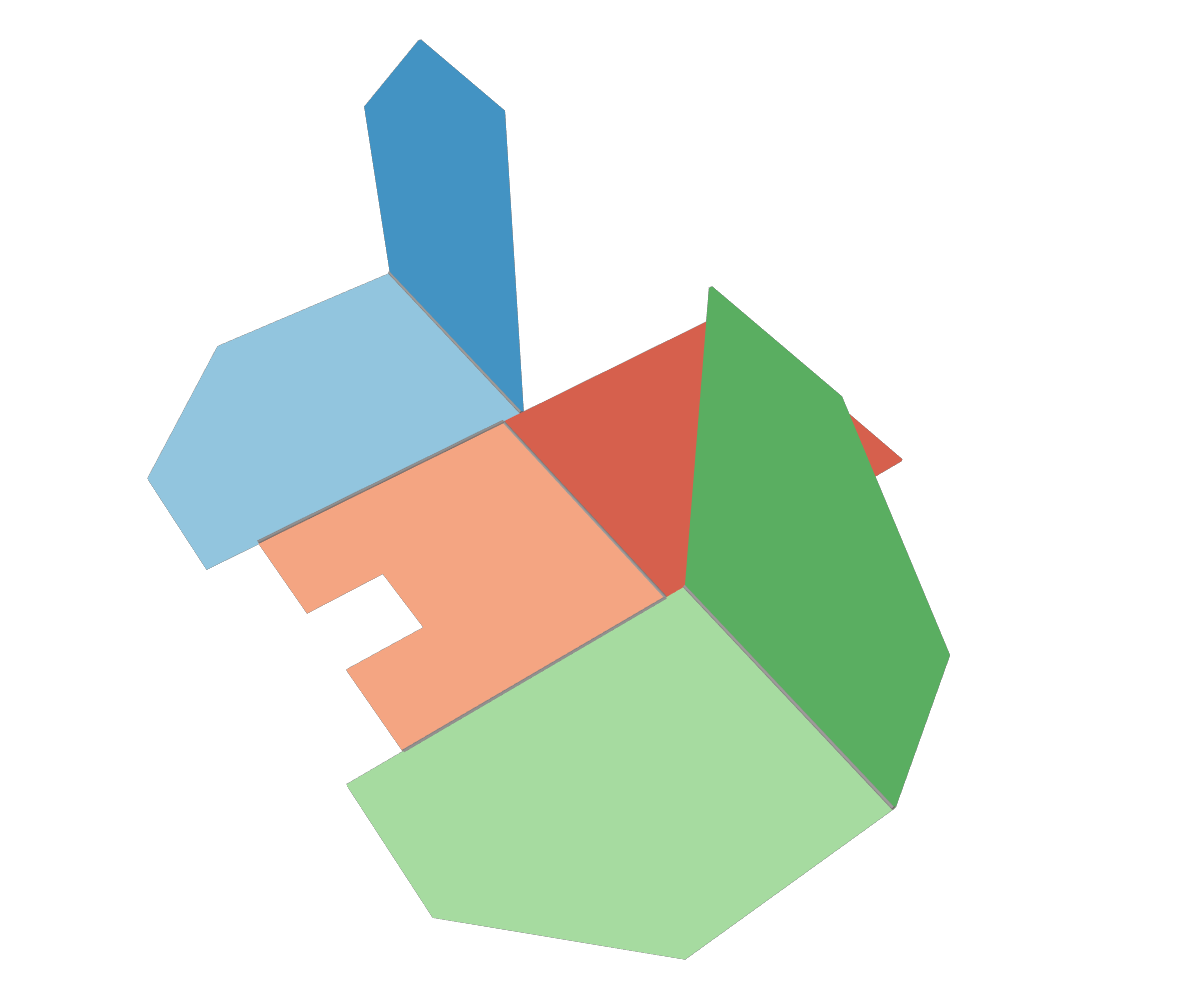
\includegraphics[height=\graphicsHeight]{sections/design/solar-array/images/deployment/ismenius-cavus/solar_array_deployment_ismenius_cavus_100.png}
		\subcaption{Port quarter and starboard quarter mid-deployment}
		\label{fig:sub:deployment-sequence-ismenius-cavus-mid-quarter}
	\end{subfigure}\hspace*{2.5cm}
    \begin{subfigure}[t]{\subfigureWidth}
        \centering
		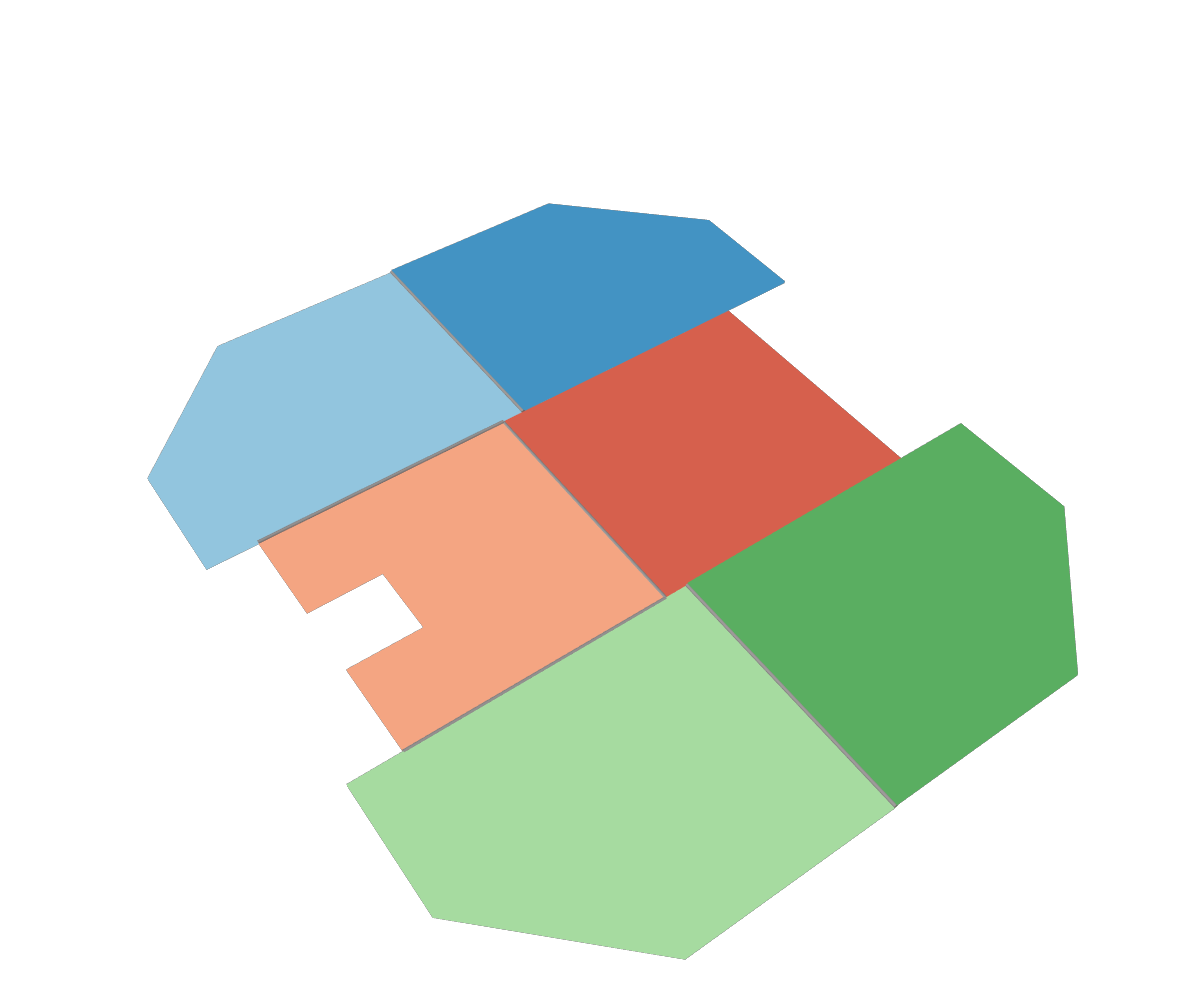
\includegraphics[height=\graphicsHeight]{sections/design/solar-array/images/deployment/ismenius-cavus/solar_array_deployment_ismenius_cavus_130.png}
		\subcaption{Completed deployment}
		\label{fig:sub:deployment-sequence-ismenius-cavus-completed}
	\end{subfigure}
	\caption{Deployment sequence of \SI{2.8}{\meter\squared} solar array at Ismenius Cavus.}
	\label{fig:deployment-sequence-ismenius-cavus}
\vspace{-2ex}
\end{figure}

\clearpage
\subsubsection{Motor Requirements}
The worst case motor torque for \ac{SA} deployment occurs when unfolding the port quarter and starboard quarter panels at Ismenius Cavus. This sequence is illustrated from Figure \ref{fig:sub:deployment-sequence-ismenius-cavus-full-bow-and-stern} to \ref{fig:sub:deployment-sequence-ismenius-cavus-completed}. The distance between the \ac{CoM} and the rotation joint is shown in Figure \ref{fig:ismenius-cavus-solar-panel-starboard-quarter-dimensions} and corresponds to $r = \SI{385}{\milli\metre}$.

\vspace{0.25cm}

\begin{figure}[h]
  \captionsetup[subfigure]{justification=centering}
  \centering
  \hypersetup{linkcolor=captionTextColor}
  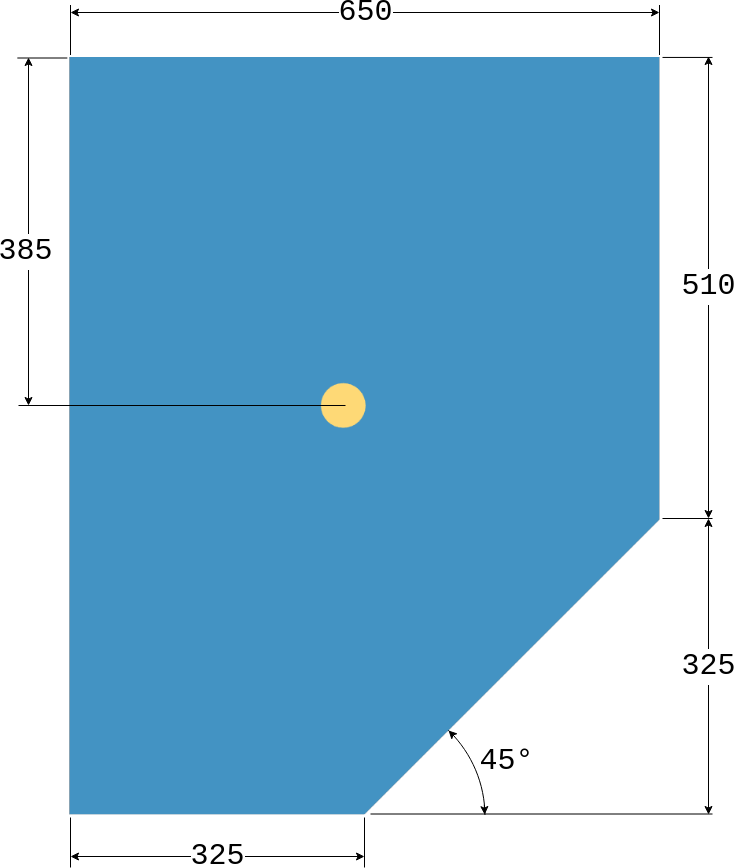
\includegraphics[width=0.45\linewidth]{sections/design/solar-array/images/ismenius-cavus-solar-panel-starboard-quarter.png}\\
  \caption[Dimensions of starboard quarter panel at Ismenius Cavus]
          {Dimensions of starboard quarter panel at Ismenius Cavus. Measurments are in millimeter. The same dimensions apply for the starboard bow, port bow, and port quarter panels. The length between the base of the panel and the \ac{CoM} is also indicated and corresponds to $r = \SI{385}{\milli\metre}$.}
  \label{fig:ismenius-cavus-solar-panel-starboard-quarter-dimensions}
\end{figure}

\vspace{0.25cm}

The distance $d_{rev}$ traveled for one revolution is:

\begin{align}
  \label{eq:solar-panel-deployment-revolution}
  d_{rev} &= 2\pi r\\
          &= 6.18 \times 0.385\\
          &= 2.38\,\si{\meter}
\end{align}

The distance $d$ traveled during the deployment sequence from Figure \ref{fig:sub:deployment-sequence-ismenius-cavus-full-bow-and-stern} to \ref{fig:sub:deployment-sequence-ismenius-cavus-completed} corresponds to half a revolution:

\begin{align}
  \label{eq:solar-panel-deployment-distance}
  d &= \frac{d_{rev}}{2}\\
    &= \frac{2.38}{2}\\
    &= 1.19\,\si{\meter}
\end{align}

The required acceleration $a'$ for a deployment duration of $t = \SI{20}{\second}$ is:

\begin{align}
  \label{eq:solar-panel-deployment-acceleration1}
  a' &= \frac{2 \times d}{t^{2}}\\
    &= \frac{2 \times 1.19}{20^{2}}\\
    &= 5.95\times\num{e-3}\,\si{ms^{-2}}
\end{align}

The gravity acceleration $g$ must be taken into account as it acts against the direction of the calculated acceleration. However, $g_{Earth} = 9.81 \si{ms^{-2}}$ is used rather $g_{Mars} = 3.71 \si{ms^{-2}}$ as a means of introducing a margin that accounts for environmental events such as wind loads. This margin also accounts for imperfections introduced by motor performance degradation factors. Furthermore, sizing motors for an Earth environment reduces design verification and validation costs by eliminating the need for vacuum chamber tests.

\begin{align}
  \label{eq:solar-panel-deployment-acceleration2}
  a &= a + g_{Earth}\\
    &= 5.95\times\num{e-3}\si{ms^{-2}} + 9.81\\
    &= 9.82\,\si{ms^{-2}}
\end{align}

The panel has a mass of 1.85 \si{\kilo\gram}, thus the required torque $\tau_{torque}$ is:

\begin{align}
  \label{eq:solar-panel-deployment-torque}
  \tau_{torque} &= m \times a \times r\\
                &= 1.85 \times 9.82 \times 0.385\\
                &= 6.99\,\si{\newton\meter}
\end{align}

The \ac{rpm} rotational speed for half a rotation in \SI{20}{\second} is:

\begin{align}
  \label{eq:solar-panel-deployment-rpm}
  rpm &= \frac{1}{2t} \times 60\\
      &= \frac{1}{2 \times 20} \times 60\\
      &= 1.5\,{\minute^{-1}}
\end{align}

Transmissions with a 1:30 reduction ratio can be obtained with a planetary gear configuration whereas reduction ratios of 1:100 up to 1:300 are achievable with a harmonic drive. Using a 1:30 transmission will require a motor that must deliver at least 0.23 \si{\newton\meter} of nominal torque and 45 \ac{rpm}. A 1:100 transmission requires a motor with at least $6.99\times\num{e-2}$ \si{\newton\meter} of nominal torque and 150 \ac{rpm}. Finally, a 1:300 transmission requires a motor with at least $2.33\times\num{e-2}$ \si{\newton\meter} of nominal torque and 450 \ac{rpm}.

\subsection{Summary}
\ac{SA} sizing for the worst case power budget of the rover's \textit{Traverse Sol} at optical depth of $\tau = 1$ does not support the use of solar tracking for the purpose of increasing traverse time. This is due to solar irradiance being mostly diffuse at high optical depths when airborn dust is responsible for scattered light. In a dusty atmosphere, an inclined \ac{SA} surface contributes negligeable energy production gains over those obtained with a horizontal configuration. Furthermore these gains are unusable on clear days due to the limited amount of daylight time available for traversing. To resolve this, the \ac{SA} sizing is instead done for the worst case \textit{Hibernation Sol} in which power draws are reduced by introducing \acp{RHU}. Assumptions, requirements, constraints, and design drivers presented in the previous section are considered in the baseline designs from which deployment sequences and motor requirements are presented. The location and stowed posture of the robotic arm should be approached differently so to enable complete folding of the panels over the rover's body. Such a configuration would significantly reduce the vertical span taken up by the stowed rover by approximately 1/3.
